\PassOptionsToPackage{unicode=true}{hyperref} % options for packages loaded elsewhere
\PassOptionsToPackage{hyphens}{url}
%
\documentclass[]{article}

\usepackage{multirow}
\usepackage{graphicx}
\usepackage[]{algorithm2e}
% \usepackage{multirow}
 
 \usepackage[round]{natbib}
\usepackage{lmodern}
\usepackage{amssymb,amsmath}
\usepackage{ifxetex,ifluatex}
\usepackage{fixltx2e} % provides \textsubscript
\ifnum 0\ifxetex 1\fi\ifluatex 1\fi=0 % if pdftex
  \usepackage[T1]{fontenc}
  \usepackage[utf8]{inputenc}
  \usepackage{textcomp} % provides euro and other symbols
\else % if luatex or xelatex
  \usepackage{unicode-math}
  \defaultfontfeatures{Ligatures=TeX,Scale=MatchLowercase}
\fi
% use upquote if available, for straight quotes in verbatim environments
\IfFileExists{upquote.sty}{\usepackage{upquote}}{}
% use microtype if available
\IfFileExists{microtype.sty}{%
\usepackage[]{microtype}
\UseMicrotypeSet[protrusion]{basicmath} % disable protrusion for tt fonts
}{}
\IfFileExists{parskip.sty}{%
\usepackage{parskip}
}{% else
\setlength{\parindent}{0pt}
\setlength{\parskip}{6pt plus 2pt minus 1pt}
}
\usepackage{hyperref}
\hypersetup{
            pdfborder={0 0 0},
            breaklinks=true}
\urlstyle{same}  % don't use monospace font for urls
\setlength{\emergencystretch}{3em}  % prevent overfull lines
\providecommand{\tightlist}{%
  \setlength{\itemsep}{0pt}\setlength{\parskip}{0pt}}
\setcounter{secnumdepth}{0}
% Redefines (sub)paragraphs to behave more like sections
\ifx\paragraph\undefined\else
\let\oldparagraph\paragraph
\renewcommand{\paragraph}[1]{\oldparagraph{#1}\mbox{}}
\fi
\ifx\subparagraph\undefined\else
\let\oldsubparagraph\subparagraph
\renewcommand{\subparagraph}[1]{\oldsubparagraph{#1}\mbox{}}
\fi
\usepackage{cleveref}
% set default figure placement to htbp
 
\def\fps@figure{htbp}
\makeatother


\author{Meng Lu }
\date{Feb 2021}
\title{An agent-based model for human activity simulation and the assessment of personal exposure to ambient air pollution}

\begin{document}
\maketitle
 
\section{Introduction}

%Chronic exposure to NO$_2$ poses a threat to public health, evidence has shown the negative effects of the NO$_2$ exposure to the cardiovascular and respiratory systems \citep{luo2016acute}. Despite public health concerns urging the attenuation of the negative effect of NO$_2$, the exact relationship between NO$_2$ exposure and our health remains unsolved. 
Highly traffic-related air pollutants such as NO$_2$ show considerable spatiotemporal variations at street levels. However, to understand the long-term or chronic health effects of NO$_2$ over a relatively large population (e.g. population of a city), most of epidemiological studies took a "static approach", which approximate the exposure as temporally averaged ambient pollutant concentrations at a person’s front-door home location. The same applies to risk assessment, the quantification of global, national, and local burden of diseases \citep{achakulwisut2019global}. It is obvious that for a spatiotemporally highly variable air pollutant, personal exposures assessed neglecting space-time activities, i.e. using concentration values at the front-door addresses, can differ considerably from personal exposures assessed accounting for human space-time activities. This difference has been reflected in several studies that attempt to account for personal or population space-time activities in exposure assessment  \citep{duan1997combination,lu2019activity,park2017individual,molter2012performance,zenk2011activity}. 

Recent studies attempting to account for space-time activities in exposure assessment over a long-term and a relatively large population commonly integrate activity models (including transportation models). The pioneered work of \cite{beckx2009dynamic} proposed to use the activity-based model to simulate hourly activities and then combine with an air dispersion model to assess exposure. \cite{beckx2009dynamic} applies an activity model called ALBATROSS \citep{ALBATROSS}, which is a transportation oriented system that simulates activities for the entire population based on activity diary data and dynamic constrains on scheduling decisions. Following this approach, a wide variety of activity models could be applied to understand human activity patterns \citep{w2016multi,miller2003prototype, shekarrizfard2017regional, deffner2016personal,gulliver2005time,dons2011impact}. These models consider a comprehensive set of space-time activity characters such as different travel means, work, education, and leisure activities, traffics \citep{w2016multi}. They are commonly parameterised by diary surveys consisting of locations visited and origin-destination schedules and estimate a continuous-time mobility track for each individual basing on general rules of human mobility patterns and space-time accessibility \citep{nguyen2011steps,gonzalez2008understanding,yang2010using,yu2006spatio,alessandretti2017multi,miller1991modelling}. Each route simulated can be contingent on, for instance, distance, safety, city infrastructure, and land use \citep{law2014measuring}. For example, \cite{shekarrizfard2017regional} assigned the predictions of a travel demand model to a road network to predict a person's hourly trajectories. For each person, the model selects a path from all possible paths by comparing the assigned travel time and the survey travel time. 

%Several attempts are made to move from static to spatiotemporally resolved exposure assessment  by   

Though activity-based models are tremendously useful in simulating human activities, their integration into a personal exposure assessment framework need to be developed to address the following challenges.  

\begin{enumerate}
    
    \item \textit{Long-term simulation}. Current models have focused on simulating hourly activities but fall short at quantifying the exposures variation over longer times, which do not consider irregular events or holidays. 
    
    %\item \textit{Dynamically assimilating activity data}. Current models depend heavily on the representative survey sampling of the real activities. %Simulations for demographic and socioeconomic groups \citep{lee2013impact} can greatly reduce model uncertainty and improve prediction accuracy.   
    
    \item \textit{Comprehensive uncertainty quantification}. An uncertainty quantification for each activity, including time schedules, travel means, and possible destination locations.
    
    \item \textit{Separating between population subgroups}. The health impacts of air pollution exposure subjects to a variety of confounders such as age, gender, and living habits. Many of these health research confounders (e.g. age) are closely related to certain space-time behaviours.  
\end{enumerate}
 
The framework developed in \cite{lu2019activity} attempts to address the first and second limitations. However, it assumes no activity information is available and therefore does not evaluate real-life cases where national micro-census data is commonly available and can provide important information about human activity patterns.  
 
We greatly extend from \cite{lu2019activity} to develop a novel human space-time activity model explicitly for exposure assessment to address the above-mentioned limitations. Our objective is to develop a model with the following features: 

\begin{enumerate}

    \item Allowing flexible inclusion of irregular (e.g. holiday) activity schedules for long-term exposure modeling, 
    
    \item Estimating or empirically specifying probability distributions for each activity, including for example departure time, travel means, possible destinations. The estimation can base on micro-census surveys using statistical modeling.
    %\item The model can conveniently assimilate any other activity-related data, using either statistical modeling or . 
    
    \item Sampling from the specified or estimated distributions repeatedly for uncertainty quantification and more accurate estimation of exposures through ensembling. 
\end{enumerate}

With this novel space-time activity model as the core component, we develop an activity-based NO$_2$ exposure assessment model consists of additionally an exposure assessment module and a temporal air pollution mapping module. The exposure assessment module takes output of the activity model, namely activity schedules and spatial locations of the activities (e.g. work locations, trip routes), and hourly NO$_2$ maps from the temporal air pollution mapping module to assess NO$_2$ exposures from each home location (\cref{fig:expflow}).     

\begin{figure}
    \centering
    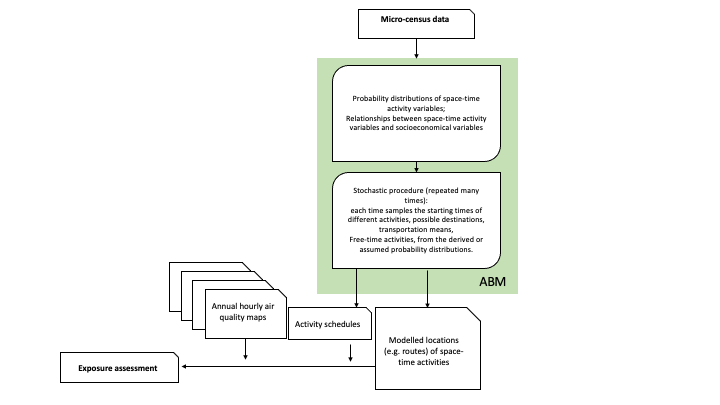
\includegraphics[width=\linewidth]{figure/exposureflow.png}
    \caption{The structure of our exposure assessment model. At the core is our agent-based human space-time activity model. ABM: agent-based modelling. }
    \label{fig:expflow}
\end{figure}
We demonstrate our activity model and exposure assessment model predictions in the Dutch city of Utrecht, for the population group university students.  

The rest of the manuscript is organised as follows: to make it concrete,  \cref{sec:data} describes the the micro-census data we used to parameterise our model. Then, we describe our space-time activity model in \cref{sec:model} and follows with the exposure assessment model in \cref{sec:exp}. \Cref{sec:result} shows the results in our study case. \Cref{sec:dis} discuss our models and the results. \Cref{sec:con} closes with a conclusion.


\section{Data}
\label{sec:data} 
We used a long-term Dutch national travel survey, OViN (2010 - 2017, followed by OVG and MON)) to demonstrate the parameterisation of each module of the model. OViN is collected by Statistics Netherlands (in Dutch: Centraal Bureau voor de Statistiek - CBS) for one-day trip-based diary. It consists of 0.3 of the Dutch population. 
%For exposure assessment we focus on the Dutch city of Utrecht.  

\subsection{Data preprocessing}
The original data of the following variables are in text, we parsed the text data to extract the range of the data and calculate a mean of the data range. The variables, their original text, and generated variables are listed below.
% Please add the following required packages to your document preamble:
 

\begin{table}[!h]
\resizebox{\textwidth}{!}{%
\begin{tabular}{l|l|l|l|l|l}
\hline
Variable       & original variable name & \begin{tabular}[c]{@{}l@{}}example of the \\ variable content\end{tabular}                           & new variables                                                                     & \begin{tabular}[c]{@{}l@{}}new \\ variable\\  value\end{tabular} & note                                                                                                                                                              \\ \hline
Trip distances & KAfstR                 & \begin{tabular}[c]{@{}l@{}}"5,0 tot 7,5 km"\\ "50 km of meer"\\ "Geen rit in Nederland"\end{tabular} & \begin{tabular}[c]{@{}l@{}}KAf\_low\\ KAf\_mean\\ KAf\_high\end{tabular} & \begin{tabular}[c]{@{}l@{}}5\\ 6.25\\ 7\end{tabular}             & \begin{tabular}[c]{@{}l@{}}"geen rit in\\  Nederland" \\ means the trip \\ is not in the \\ Netherlands \\ and is not \\ considered \\ in this study\end{tabular} \\ \hline
Income         &                        &                                                                                                      &                                                                                   &                                                                  &                                                                                                                                                                   \\ \hline
Age            &                        &                                                                                                      &                                                                                   &                                                                  &                                                                                                                                                                   \\ \hline
...            &                        &                                                                                                      &                                                                                   &                                                                  &                                                                                                                                                                   \\ \hline
\end{tabular}%
}
\end{table}

\section{Human space-time activity model}
\label{sec:model}

The most important task of the human space-time activity model (HSTAM) is to generate activity schedules for each home locations. The process is repeated several times (each repetition is called an iteration) for uncertainty quantification and improving the prediction accuracy of the exposure assessment following the framework proposed in \cite{lu2019activity}.  In each interaction, the major steps are:   

\begin{enumerate}
    \item Specify the distribution of travel distances based on the survey data if the distribution is not pre-defined. 
    \item Sample from the distribution of the travel distances to choose a destination location from all possible destination locations.
    \item Based on the distance, it samples a travel mean according to the relationships identified between travel mean and travel distances, for different population groups  (e.g. old people, students) and travel purposes (e.g. going to work).
    \item A route is queried from OpenStreetMaps for the estimated travel mean. For example, a walk path is queried if the travel mean is by foot.  
    \item Based on the travel distances and travel mean, the duration is deducted. 
    \item Based on the duration, the end time of a trip or the start time of the next trip is estimated. 
    \item If the previous trip is not on a road, the start time of the trip is generated with a distribution. For example, the default departure time to work in our model is sampled from a Gaussian distribution with mean 8 (i.e. 8 am) and standard deviation 0.2. 
    \item The free time activities are randomly sampled from a set of activities, for example, staying at home or take a walk. 
\end{enumerate}

\Cref{fig:detail} illustrates how an activity schedule is generated. 

\begin{figure}
    \centering
    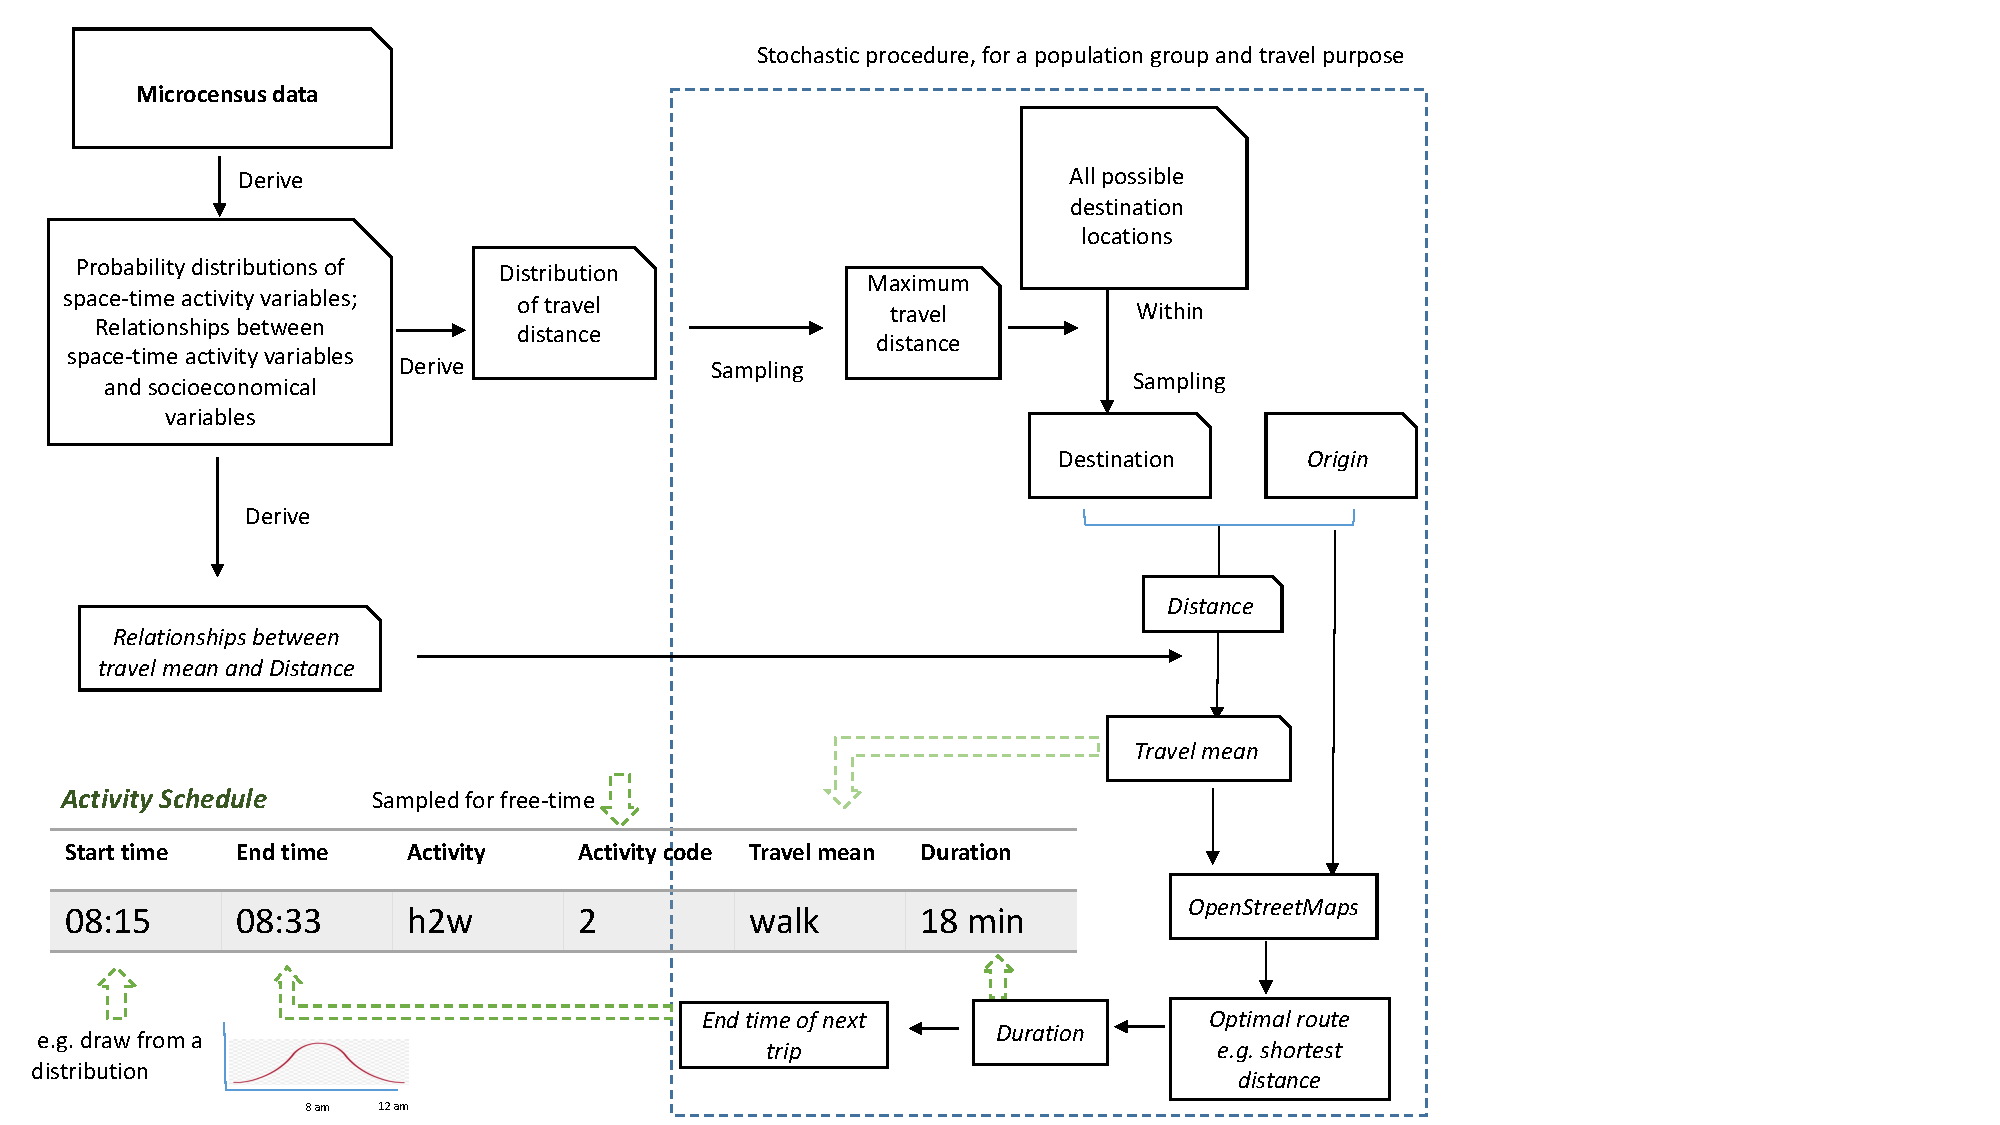
\includegraphics[width=\linewidth]{figure/scheduleflow_noenrich.pdf}
  \caption{Procedure of generating activity schedules using the human space-time activity model}
    \label{fig:detail}
\end{figure}

\subsection{Input and output of the model}

The input of the HSTAM consists of 1) home locations to estimate. 2) All the possible destination locations for each destination type (e.g. all the work locations, all the school locations). 3) A table indicating the probability each travel mean is taken for different distances and for different population groups and travel purposes. 4) The distributions of the travel distances for certain population groups, either pre-defined by the user, i.e., the distribution is the input, or predicted from survey data, i.e. the survey data is the input.
 

The HSTAM generates activity schedules and spatial locations and tracks of the activities, for each iteration and each individual. The activity schedule consists of, for each trip, a start time, an end time, the travel mean, the duration, as well as the activity name and a corresponding code. \Cref{tab:sche} shows an example. The spatial locations of the activities, as well as the properties of trips, including the speed, means, duration of a trip, the total number of locations a destination is drawing from, are stored in the OGC GeoPackage format. 

\begin{table}[]
\resizebox{\textwidth}{!}{%
\begin{tabular}{cccccc}
\\[-1.8ex]\hline 
\hline \\[-1.8ex] 
start\_time & end\_time & activity   & activity\_code & travel\_mean          & duration                   \\ \hline
0.0         & 7.06      & home       & 1              & \multirow{7}{*}{foot} & \multirow{7}{*}{335.55672} \\
7.07        & 7.17      & h2w        & 2              &                       &                            \\
7.18        & 16.14     & work       & 3              &                       &                            \\
16.15       & 16.23     & w2h        & 2              &                       &                            \\
16.24       & 17.73     & home       & 1              &                       &                            \\
17.74       & 19.73     & free\_time & 1              &                       &                            \\
19.74       & 23.9      & home       & 1              &                       &     \\ \hline                      
\end{tabular}%
}
\caption{An example of activity schedules. h2w means "home to work", and w2h means "work to home". The "bicycle" indicates the transportation mean, which is generated from the activity model. The integer part indicates hours, and the digits indicate minutes in percentage, e.g., 9.89 is at around 9:54 am (54 = 89*0.6).}
\label{tab:sche}
\end{table}
 
\subsection{Probabilistic components}
This section describes the details of generating the components that are probabilistic.  
\begin{enumerate}
\def\labelenumi{\arabic{enumi}.}
\item
  Activities:
  \emph{Work-day activities:} 1) home, 2) home to work, 3) work, 4) work
  to home, 5) sports. The assumption for sports is that it occurs in the
  morning or evening, and it occurs either 1 hour before departure to
  work or 1 hour after come back home from work.

  \emph{Weekend activity}: 1) shopping, 2) random walk 
\item
  A \textbf{probailistic} model: the components below are probabilistic,
  and the distributions can come for activity surveys or literature.

  1) \underline{Time schedule:} please see section 2 for the activities.
  The departure times to work and back from home are probabilisitic. By
  default, a gaussian distribution is used (e..g with mean 8 and
  standard deviation 0.5 for going to work). In our implementation, the
  distributions of departure times are fitted (characterised) from human
  activity surveys (please see section 4 below). The distributions are
  fitted for each population group.

  2) \underline{Unknown destination locations:} For large-population
  activity modeling, it is commonly the case that the specific
  destination location (e.g. work location, sport centres) are unknown
  for each individual. However, the information for the entire locations
  (e.g. sport centres, work buildings, universities, schools) are
  becoming more comprehensive. In many countries, this part of
  information can be acquired from OpenStreetMaps. In this study, we
  select potential locations by proabilisticly sampling the maximum trip
  distance and only randomly select locations within the Euclidean
  distance of the maximum trip distance. If there is no destination
  points within the sampled maximum trip distance, the nearest
  destination point is used. The number of total selected destination
  points serve as an uncertainty indicator in the situation of unknown
  destination locations, in each simulation run.

  3) \emph{\underline{Means of commuting}} (currently: (train),
  autovehicles (car, bus, tram), bike, on foot): are deteremined based
  on travel distance. Based on the population group (e.g. school
  student) and the travel purpose (to school), the probability that a
  certain travel mean is taken is calculated (e.g. 0.3 for on foot and
  0.6 for biking, 0.1 for taking a bus or car and 0 for others),
  according to which a travel mode is sampled in each simulation. The
  commuting routes are queried from OpenStreetMaps.

  Note: {[}How is the train route calculated? If an agent (person) takes
  a train, it is assumed he/she will firstly walk or cycle to the
  nearest train station, and get off at the train station closest to the
  destination location. (\emph{to be considered}). I intend to firstly
  model within the Utrecht city, so all the destinations should be
  constrained to a certain distance, therefore the mode: train has a
  very small probability. This model may also be remove, then in
  implementation i can simply replace train with autovehicles{]} .
\item
  Implementation:

  Population group implemented are: school student (U17) , University
  student (students older than 18 years old, Uni), part-time worker
  (PW), full-time worker (FW).

  There is a conceptural default implemented in our model which is
  described in table 1. In our case-study (Utrecht) implementation, they
  are characterised from Dutch national activity surveys (OVin). The
  process is: 1) we select a profile (e.g. Univeristy student) and a
  purpose (e.g. go to work), 2) we fit the distribution of the selected
  data. 3) At each simulation, we sample one value from the
  distribution. Specifications are described below:

  \textbf{Destination location selection:}
\end{enumerate}

\begin{itemize}
\item
  Default: randomly pick a location.
\item
  OVin: probability counted from means of \emph{commuting vs. distance}.
  for each population group (but not specified with travel purpose).
\item
  Profile implemented: School students (U17), University students (Uni),
  PW, FW; for going to work (including all functional non-residential
  buildings, data same as the Utrecht paper), going to universities
  ((locations from OSM), going to schools (locations from OSM).

  \textbf{Means of commuting}:
\item
  Default: conceptural probabilistic model for going to work.
\item
  OVin: probability counted from means of \emph{commuting vs. distance}.
  for each population group (but not specified with travel purpose).
\item
  Profile implemented: School students (U17), University students (Uni),
  PW, FW.

  \textbf{Departure time to work:} 
\item
  Default: gaussian model with mean 8 and standard deviation (SD) 0.5.
\item
  OVin: Distribution characterised: departure time (KVtijd). 
\item
  Profile implemented \emph{(Todo)}: School students (U17), University
  students (Uni), PW, FW. 
\end{itemize}

\subsection{Activity modeling using Ovin}
The example below shows how we model the profile group: school student (U17). The activities considered are 1) going to school, 2) staying at school, 3) going back home, 4) going to a sport center, 5) going back home.  


%Firstly, we characterise the distribution of the distances between home location and a work location. 
\textbf{Selecting the locations of school and sport centres.}

We demonstrate here the selection of the school location for each individual considered, selecting the location of a sport centre follows the same procedure.   
\begin{itemize}
    \item Step 1: histogram analysis and model fitting. \\ From the histogram of the travel distances between student's home location and work (i.e. school) location \cref{stu_work_hist}, we can observe that the original distribution is log-normal or power law. The log transformed distribution is visually close to a normal distribution. We therefore fit both models and at last decided on a log-normal. We conducted a Shapiro test to prove the log-normal distribution.  
    
    \item Step 2: distance sampling. \\ In each simulation step, we randomly sample a distance from the fitted log-normal distribution.
    
    \item Step 3: Select candidate/potential destinations. \\ The sampled distance is regarded as the maximum travel distance (MTD), all the possible locations (i.e. all the schools) within the Euclidean distance of the MDT are considered as the "candidate destinations". (As the actual routes have a longer distance, this can be seen as an a bit conservative way of selecting potential destinations). 
    
    \item Step 4: Randomly sample one location from all the potential destinations.
    
\end{itemize}
\begin{figure}[!h]
    \centering
    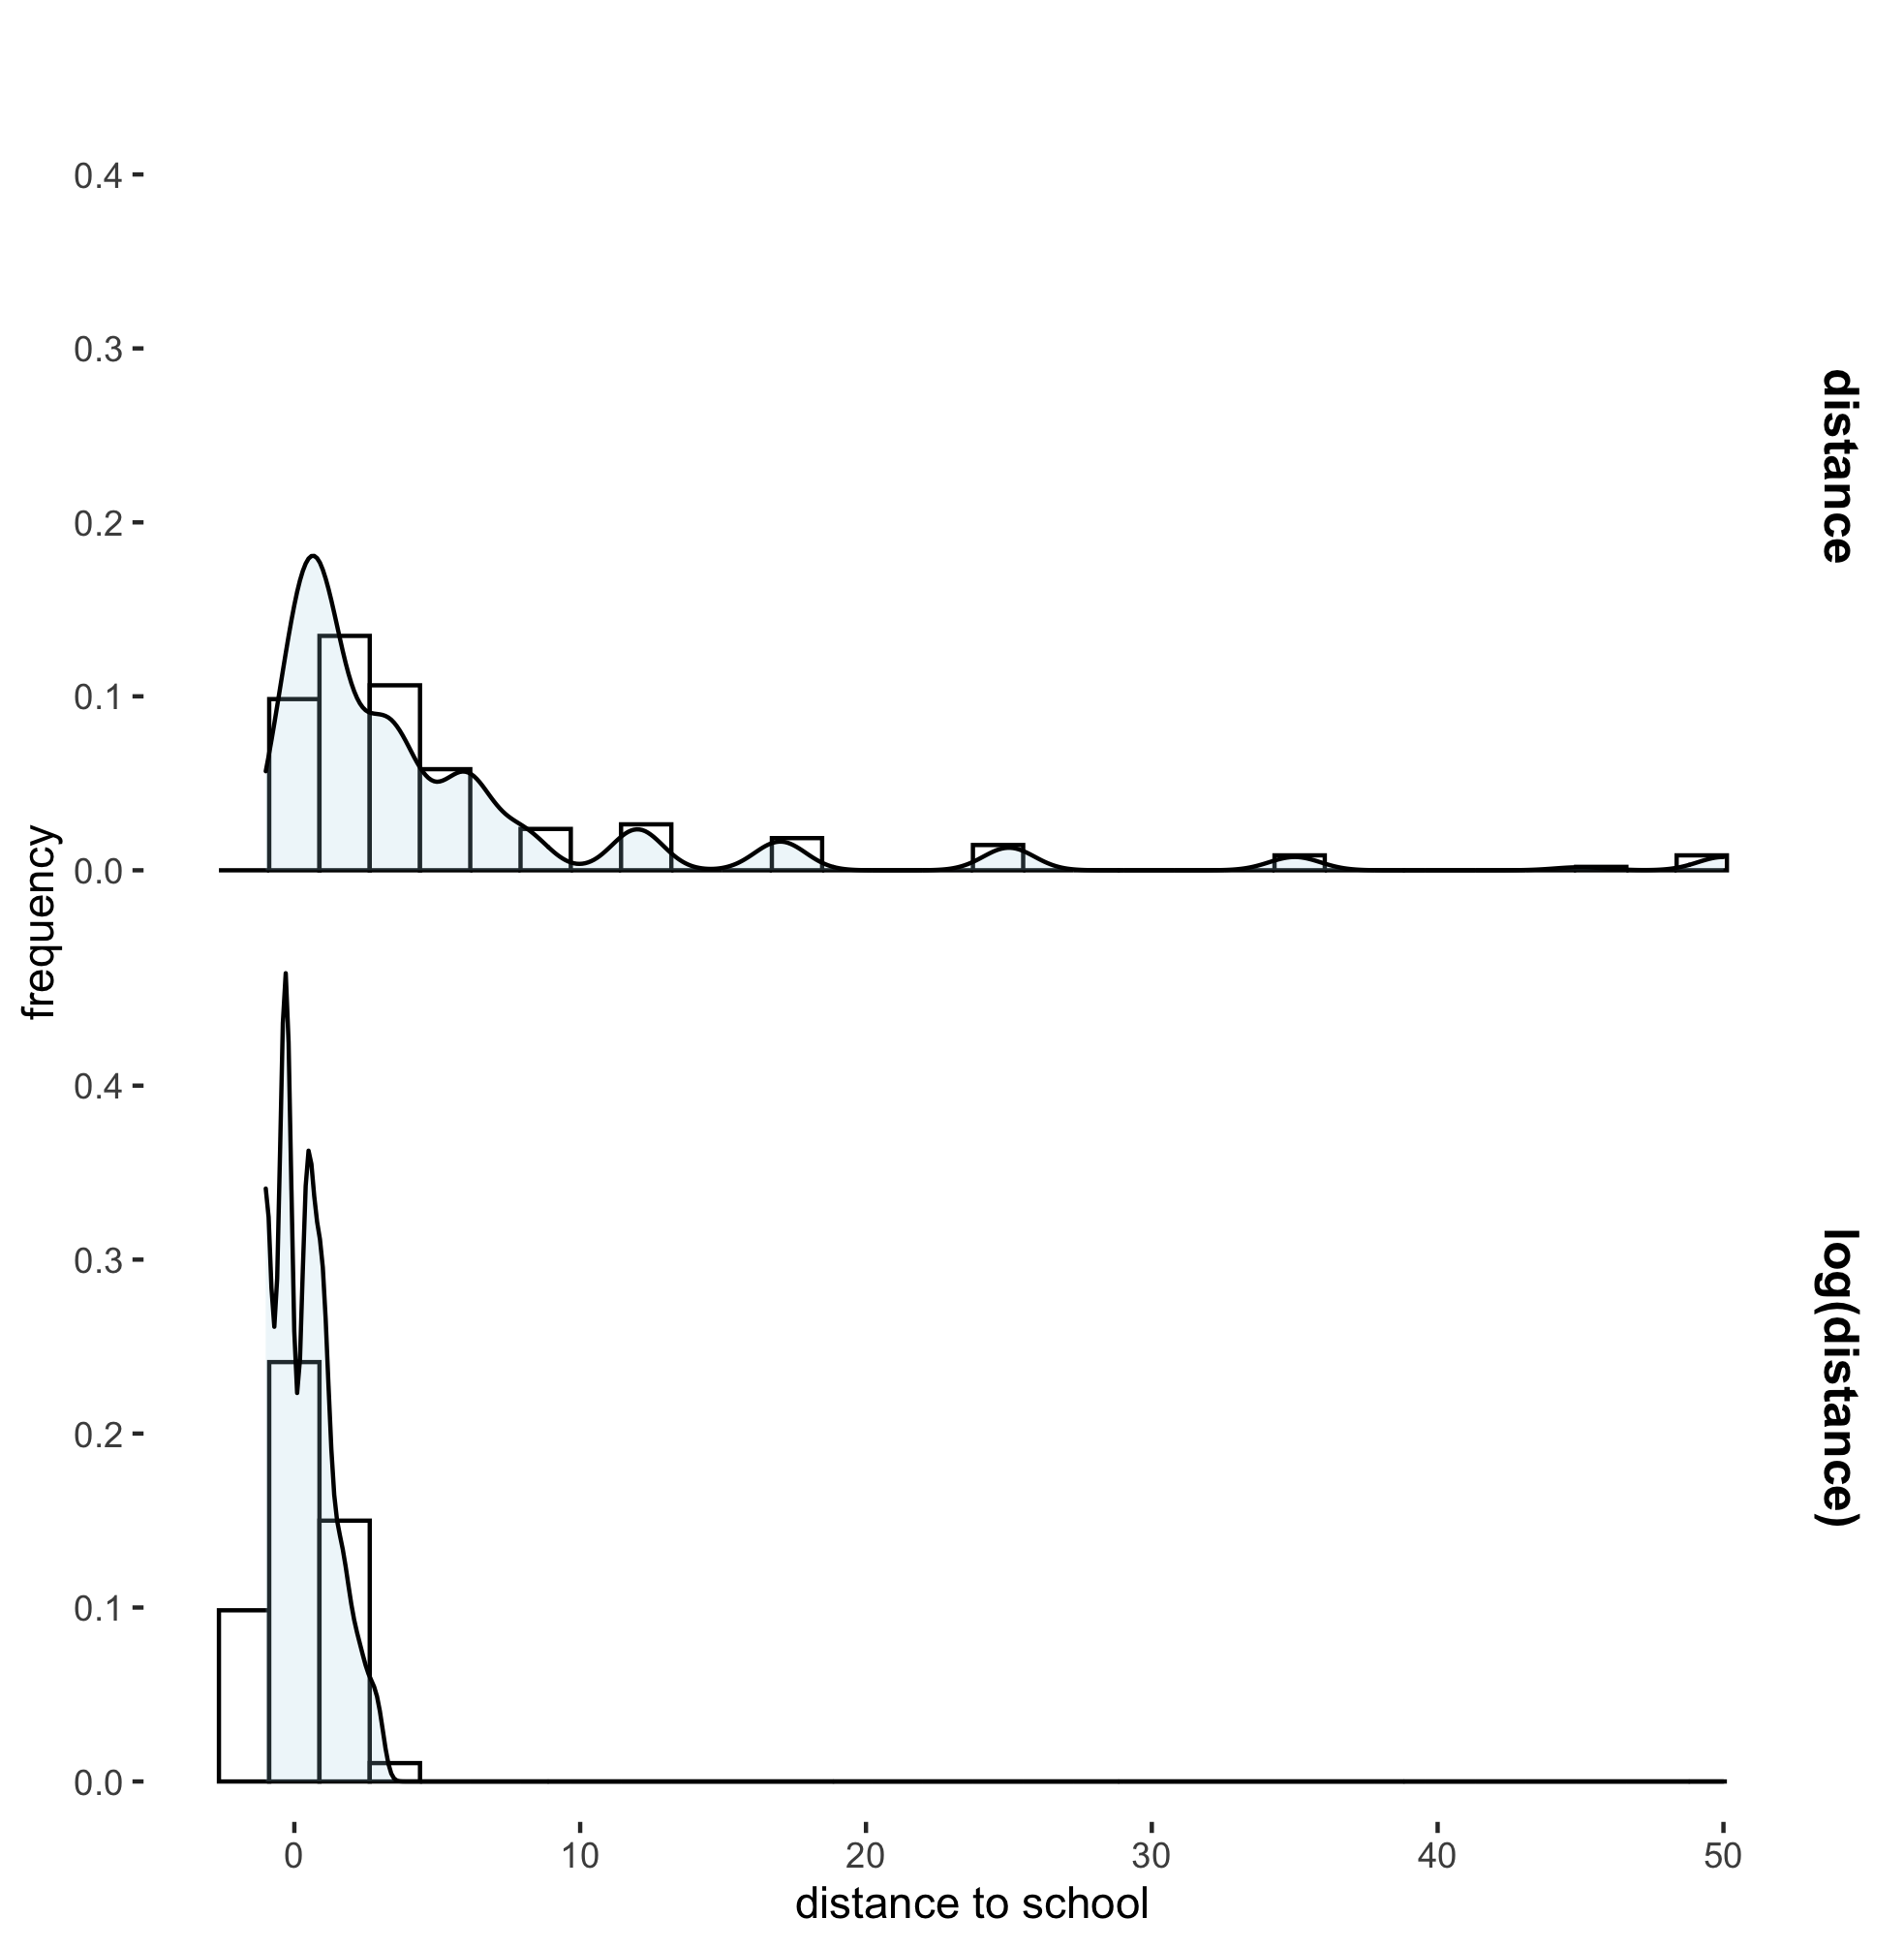
\includegraphics[width=8cm]{figure/ditance_to_school.png}
    \caption{Histograms and density plots of the distances between students' home location to work locations. }
    \label{stu_work_hist}
\end{figure}

\begin{figure}[!h]
    \centering
    \includegraphics[width=8cm]{figure/buffer.png}
    \caption{Example of selecting a sport location. The triangles indicates all the sport facilities. Only the locations within the maximum travel distances are considered, i.e. the green triangles within the buffer. And from them, one of the location is randomly sampled, marked as the \textit{Ping-pong racket and ball}. }
    \label{buffer}
\end{figure} 

An alternative way to replace step 3 and 4 is to calculate the distances between the original location and all the destination locations, and directly sample a location. This method is computationally much more intensive. 

\textbf{Choosing the transportation mean}

Now we have the home location and the destination (i.e. sport centre, school) locations, the second step is to choose the transportation mean based on the trip distance. 

\begin{itemize}
    \item Step 1: regroup transportation means and the travel distance range. \\ We regrouped the transportation means to bike, train, walk, and auto vehicles, which include all the other transportation vehicles (bus, tram, car,...). We regrouped the travel distance range as shown in \cref{stu_mode_dist}. 
    
    \item Step 2: calculate the probabilities of the transportation means within each travel distance range. \\ we count for each travel distance range the incidence of each transportation mean, and divided by the total incidence of each travel distance range to obtain the probability (of the transportation mean in each travel distance range).
    
    \item Step 3: sample the transportation mean. At last, based on the travel distance, which is calculated from the OpenStreetMap walking routes \footnote{we use the walking routes as this is commonly shorter than other routes, if this is already long, then the person has a very high probability of taking a car} based on the original location (e.g., home) and the destination (e.g., school), we sample a transportation mean given the probability.   
    
\end{itemize}

\begin{figure}[h]
    \centering
    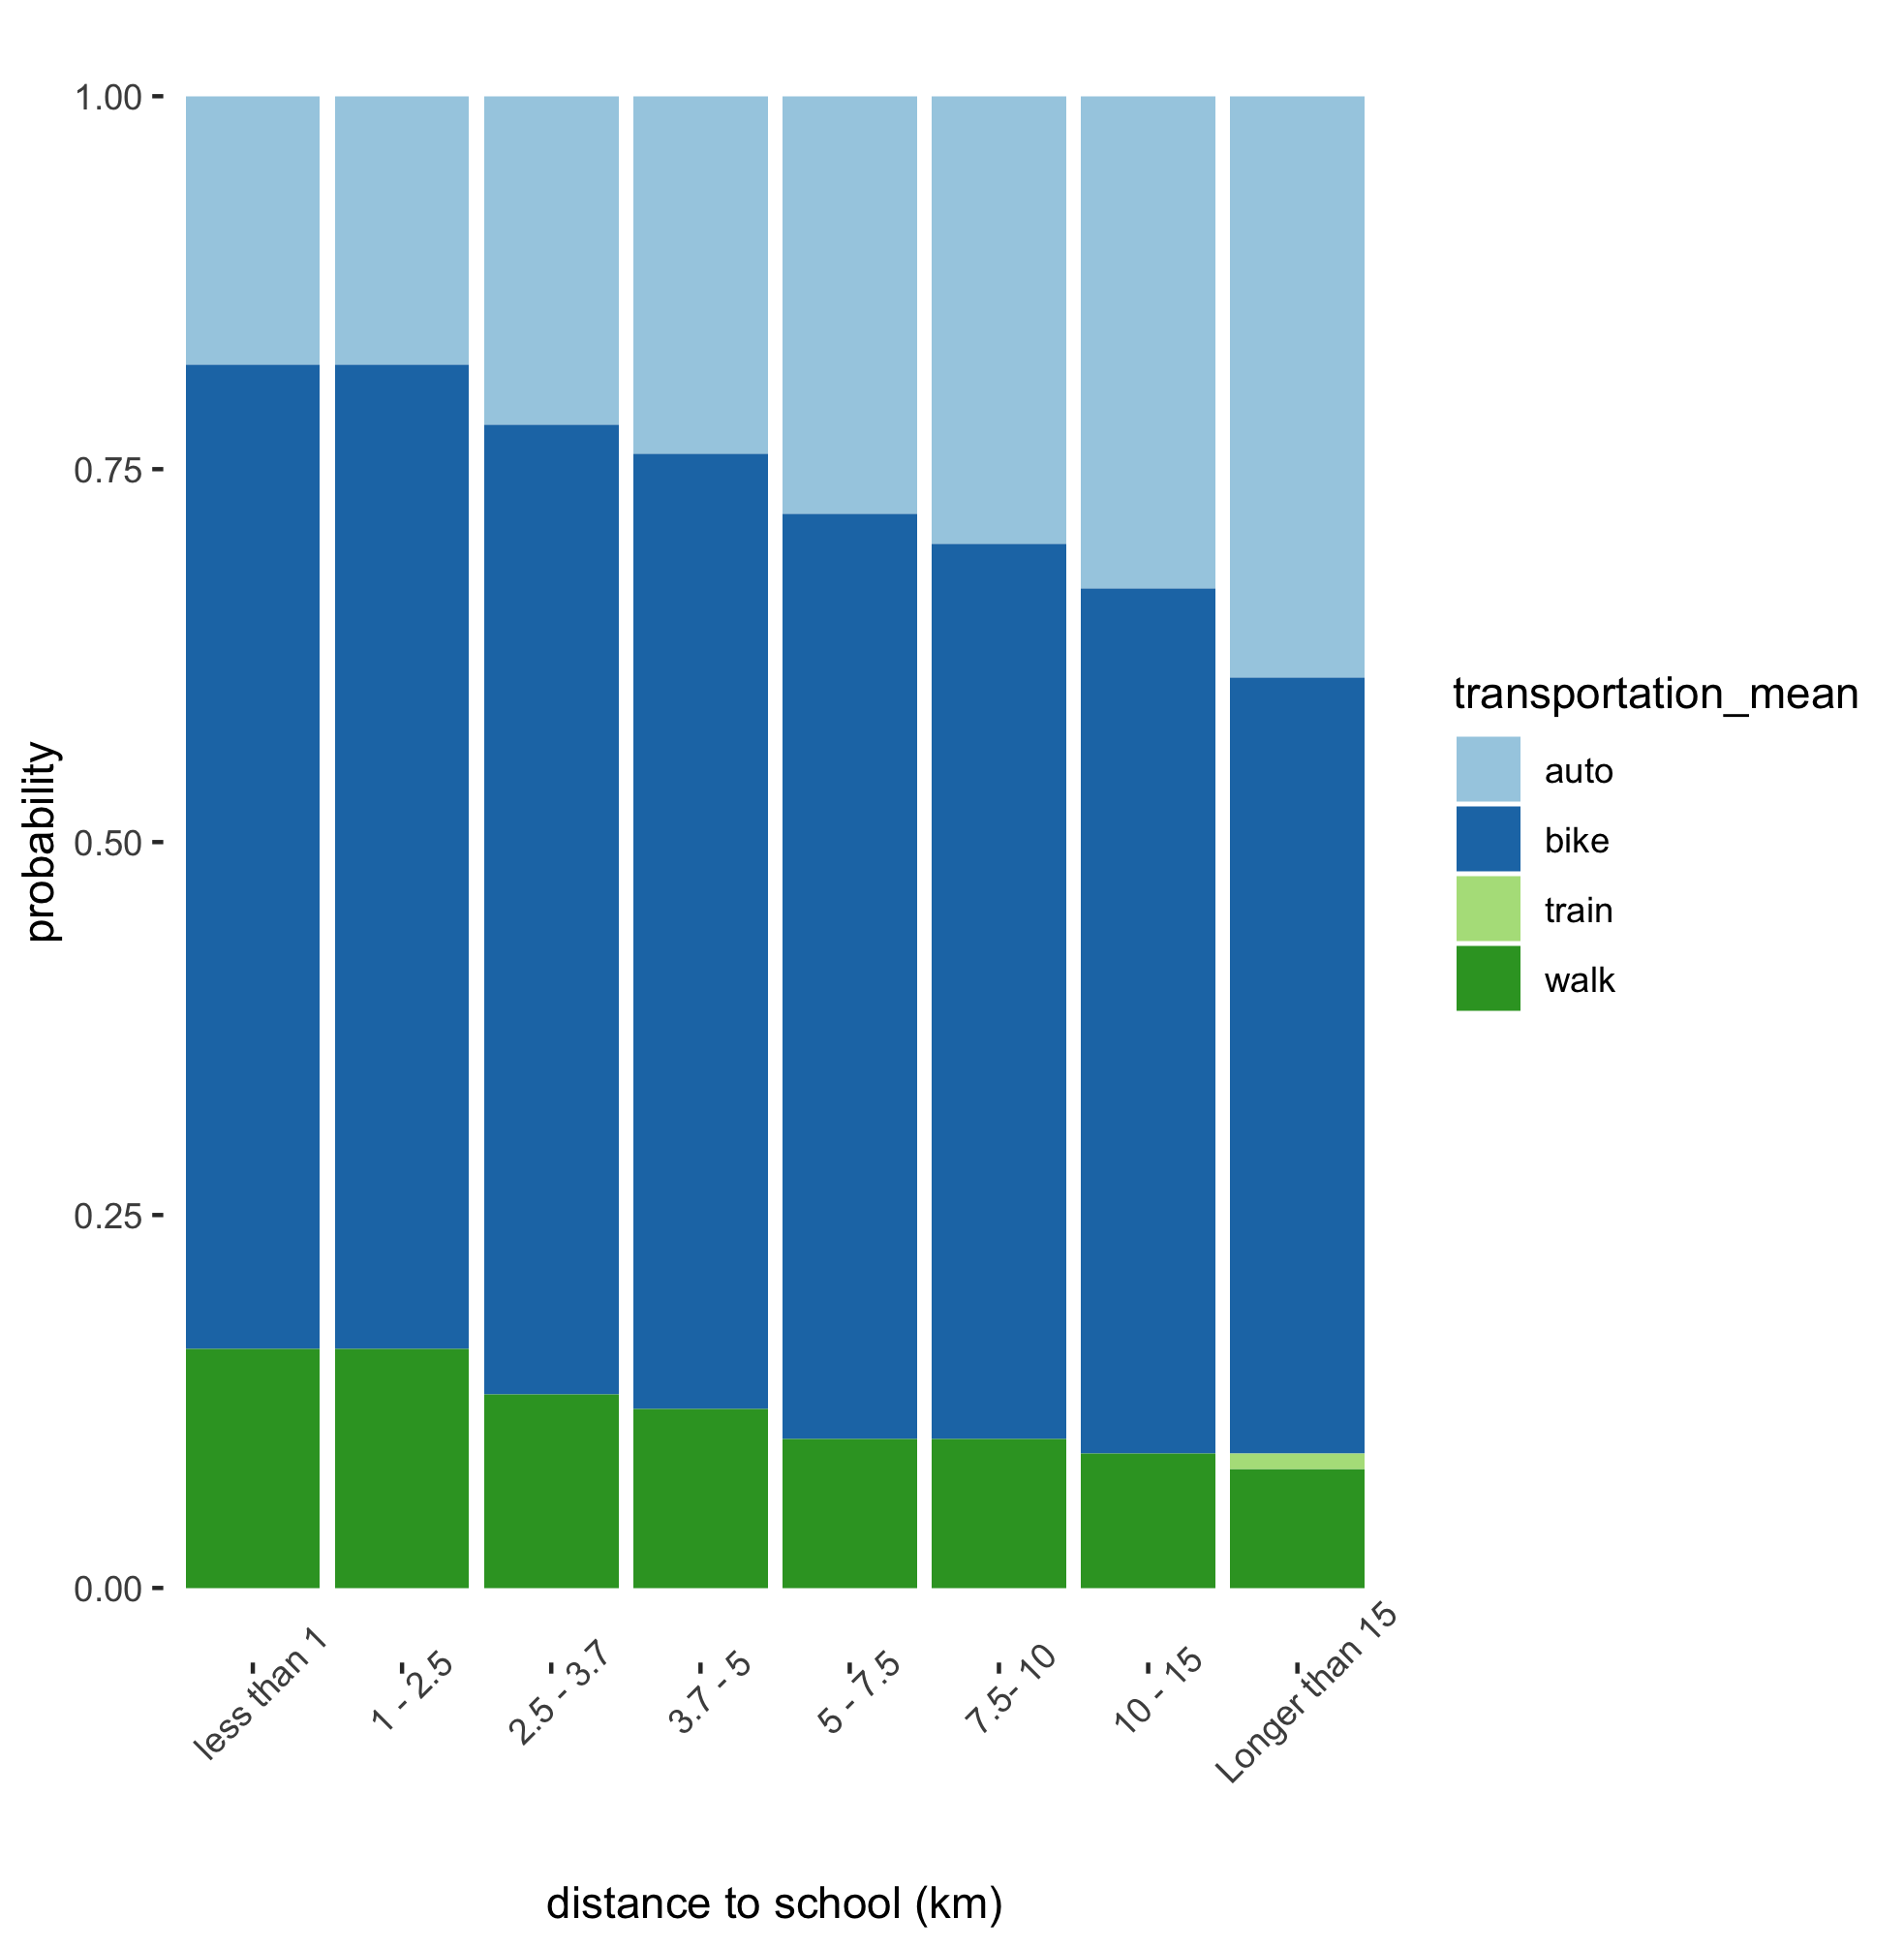
\includegraphics[width=8cm]{figure/ditance_vs_transmean_schoolstud.png}
    \caption{Probability of the transportation mean with regard to trip distance ranges for students (U17). The trip distance ranges are re-scaled from the original travel distance. The transportation means are re-grouped from the transportation means in the Ovin survey.}
    \label{stu_mode_dist}
\end{figure} 

\textbf{Generating the activity schedule and geospatial information (e.g. routes)}

Based on the transportation mean, we query the OSM route and the travel time accordingly. E.g. if the transportation mean is "bike", then we use the bike routes. With the travel time to each destination, we can complete our schedule with the starting time and the ending time of each activity. There are two ways of generating the time of going to school, as described in the section \textit{Time Schedule} above. An example simulated schedules look like \cref{schedule,schedule2}. An additional "Geometry" will be added to link the activity with the geographical points (e.g. front door location), lines (e.g. routes), or polygons (e.g. buffers). An example is shown in \cref{exampleroute}.
\begin{figure}[!h]
    \centering
    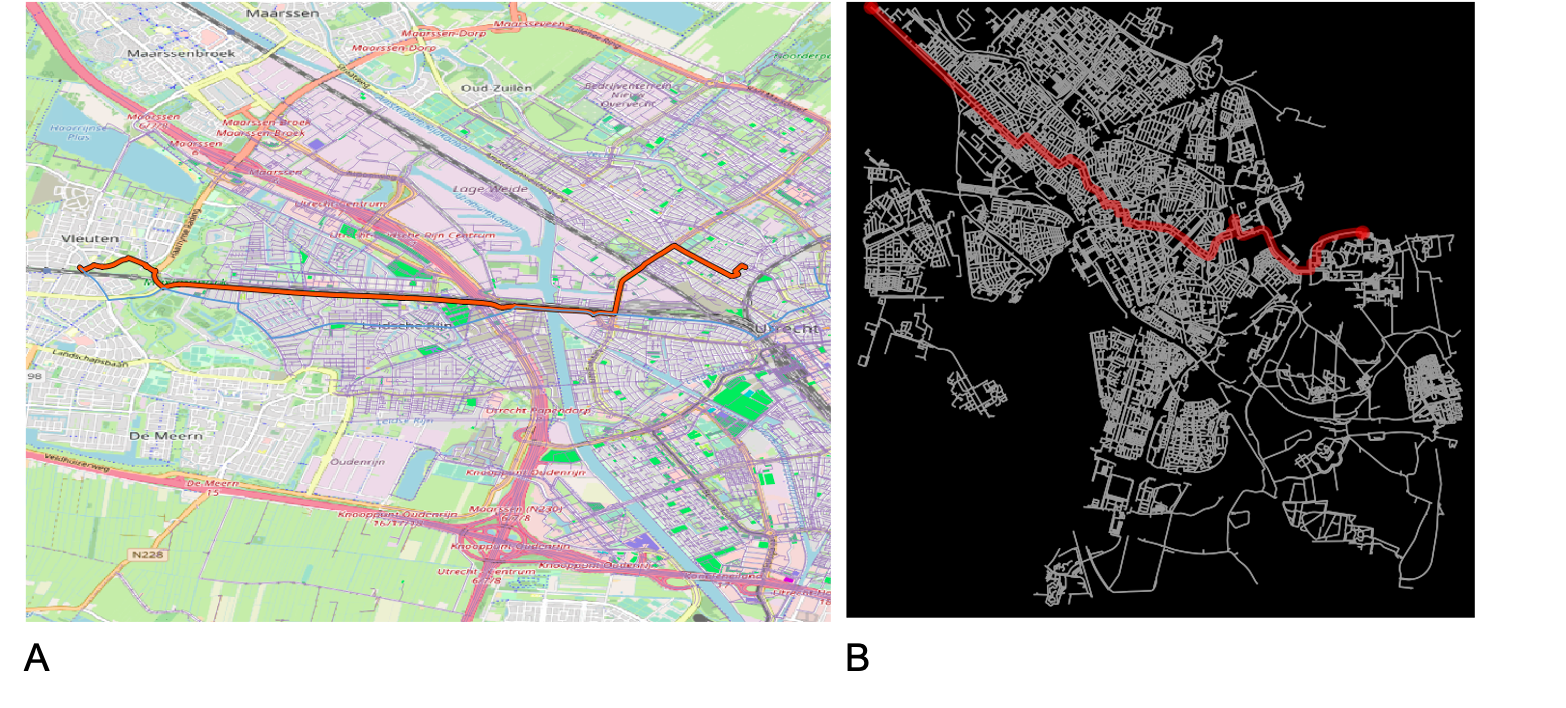
\includegraphics[width=10cm]{figure/route.png}
    \caption{Example of routes queried from the OpenStreetMaps of an individual taken from home to work, in the city of Utrecht. A route with the shortest travel time is selected for travelling on drive ways, and a route with shortest travel distance is selected for on bike and walk ways. A: bike route, B: drove route.}
    \label{exampleroute}
\end{figure}
%


\section{Exposure assessment model}
\label{sec:exp}
 Based on the activity model, we develop an Exposure assessment model, which consists of three components:
 \begin{enumerate}
     \item The activity model for generating the activity schedules and spatial locations and routes. 
     %The activity schedules and spatial destination locations and routes can be generated based on literature, activity survey, activity diaries. 
     
     \item A machine learning-based statistical model for mapping annually aggregated hourly NO$_2$.  If temporal air quality maps are available, this module can be skipped.
     
     \item An exposure calculation module for spatiotemporal aggregation of the NO$_2$ concentration over the spatial locations of the person. If the activity model is run $N$ time to simulate different schedules and spatial locations for each person, the  exposure is calculated $N$ times for the exposure of each iteration. By default, we use the mean of exposure calculated in the $N$ iterations as the final exposure assessed.   
 \end{enumerate}

An example is given in \cref{exp_act}
\begin{figure}[!h]
    \centering
    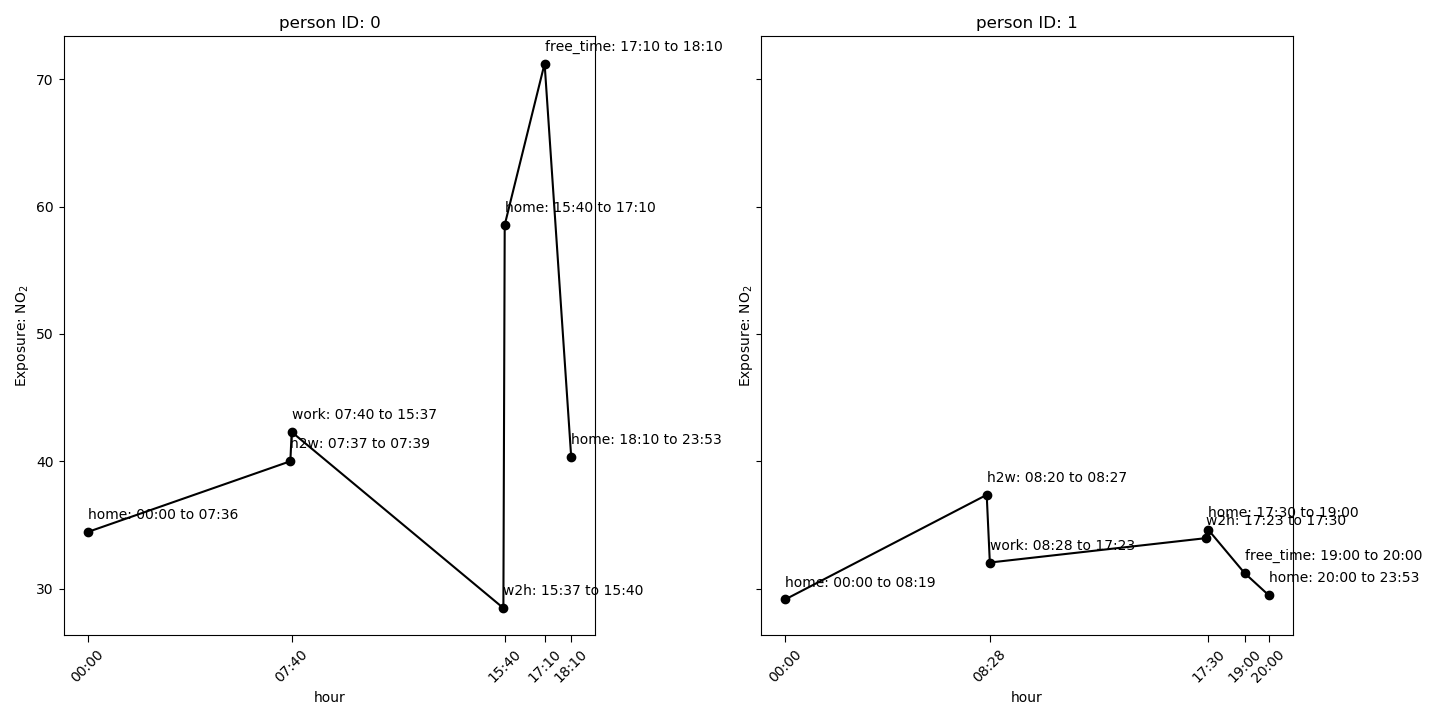
\includegraphics[width=12cm]{figure/exposure_act1.png}
    \caption{Example of assessed average exposure during each activity, in a single simulation instance. NO$_2$ exposure in $\mu g/m^3$ }
    \label{exp_act}
\end{figure}

\subsubsection{NO$_2$ prediction model}
We used the lightGBM (light gradient boosting machine) \citep{ke2017lightgbm} to predict hourly air quality from ground station measurements of Germany and Netherlands and geospatial predictors. LightGBM is a tree-based gradient boosting framework, which uses histogram-based algorithms to bin the continuous values of each feature \citep{ke2017lightgbm}. We compared the performance of LightGBM with XGBoost \citep{chen2015xgboost} with optimised hyper-parameters, and found the LightGBM obtained a slightly higher prediction accuracy (about 5\% lower in RMSE).

The predictors we used are highways, primary roads, local roads and industry areas in 100, 300, 500, 1000, 3000, 5000 m buffers; nightlight in 495, 750, 1050 m buffers; Tropomi L3 product (10km); elevation (30m); monthly wind speed and temperature of 2017 from the ERA-5Land simulation model. [details will be added].


\subsubsection{Exposure assessment model}
The exposure is assessed for each individual and scans over each activity in the activity schedule. The pseudo-code \cref{pc_e} shows the process. 
 
\begin{algorithm}[H]
 \KwData{temporal NO$_2$ maps, for each agent activity schedules and spatial locations associated with each activity in the schedule.}
 \KwResult{exposure assessed for each activity and for each person.}
 
 \For{each agent}{
 initialization\;
 exposure\_activity = 0 
 
 \For{each activity}{ 
    exposure\_activity $+=$ NO$_2$\_of\_corresponding\_time\_over spatial\_locations\_of\_the\_agent $\times$ activity\_duration
 }
exposure\_agent = exposure\_activity /time\_of\_all\_activities   
 }
 \caption{Exposure calculation, exposure\_agent indicates exposure calculated for each agent, exposure\_activity indicates exposure calculated for each activity in the schedule for each agent.}
 \label{pc_e}
\end{algorithm}


\section{Result}
\label{sec:result}

\subsubsection{Annually aggregated hourly prediction of NO$_2$}

\Cref{con} shows hourly NO$_2$ predicted using Light GBM. The error matrix is shown in table X.  

\begin{figure}[h]
    \centering
        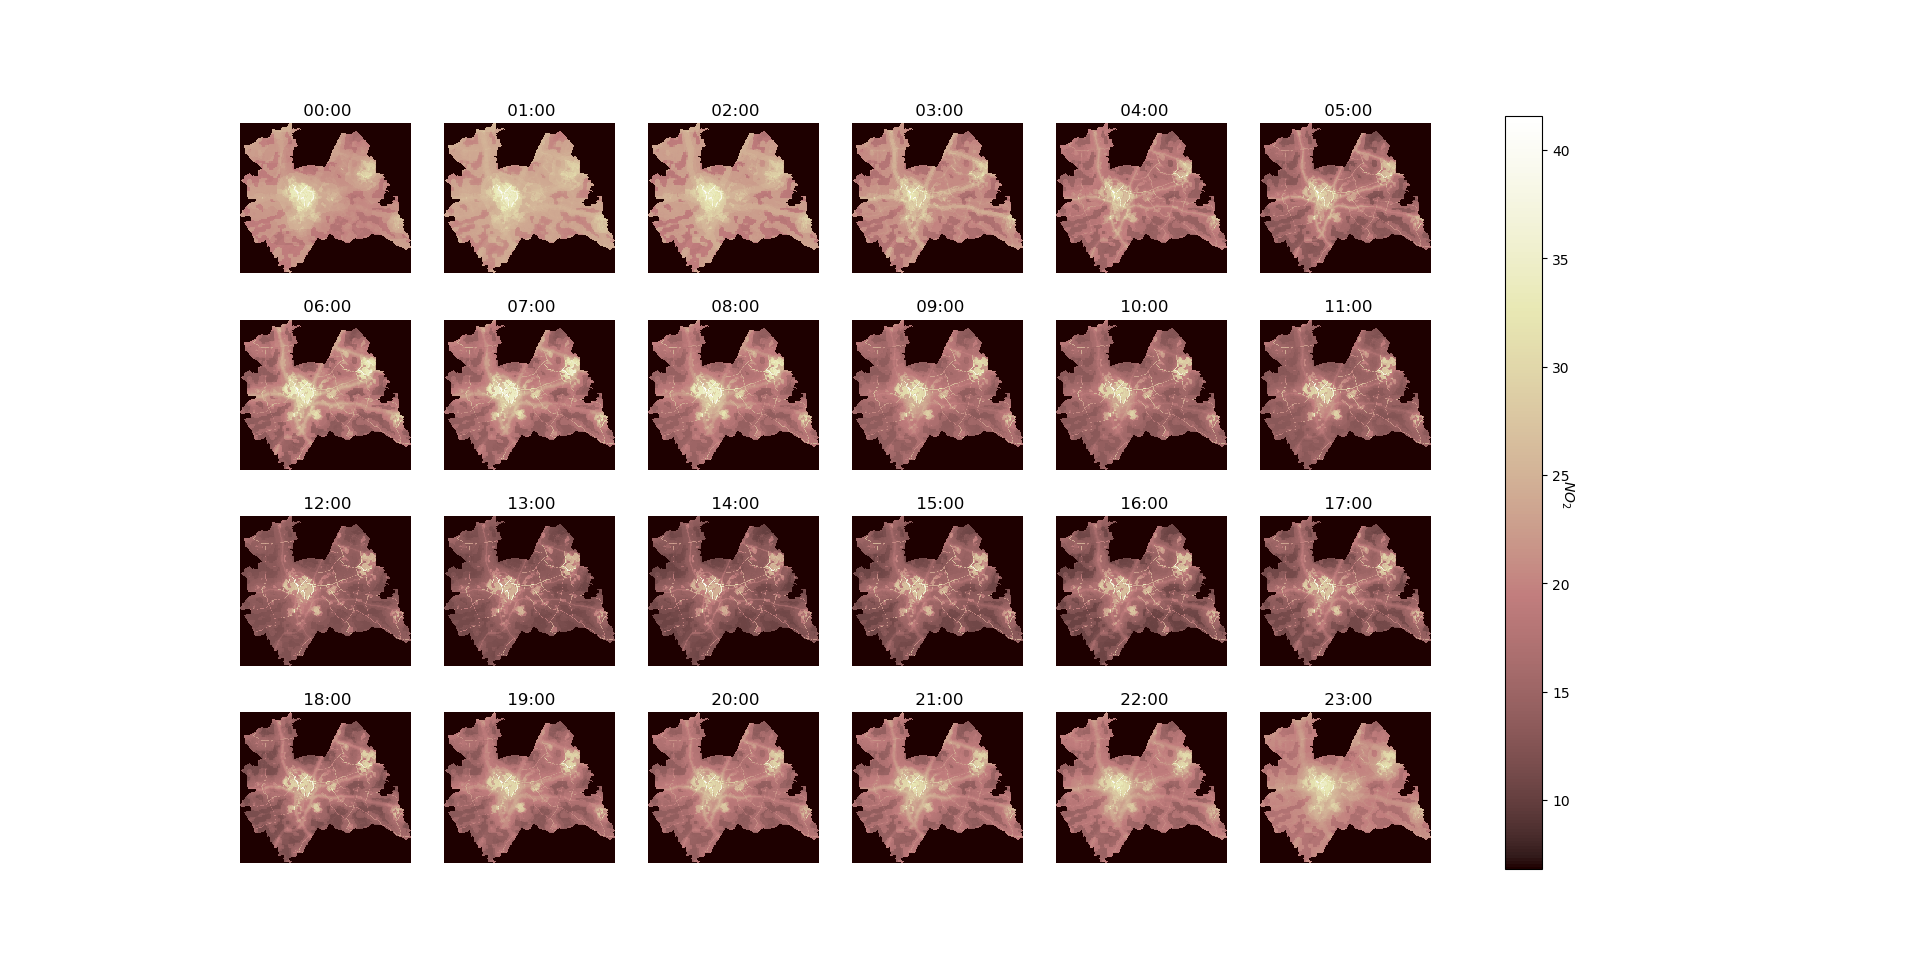
\includegraphics[scale = 0.3]{figure/prediUt.png}
    \caption{annually aggregated hourly NO$_2$ ($\mu g / m^3$) predicted for Utrecht.}
    \label{con}
\end{figure}

\subsubsection{Exposure calculated}

A example of exposure assessed using the model, for one of the activities: home to university \cref{sims}. The exposure assessed using true location is shown for comparison. It can be observed that the exposure calculated using the proposed model is close to the exposure calculated using the true location. Multiple simulations provide us an uncertainty measure.  
\begin{figure}[h]
    \centering
    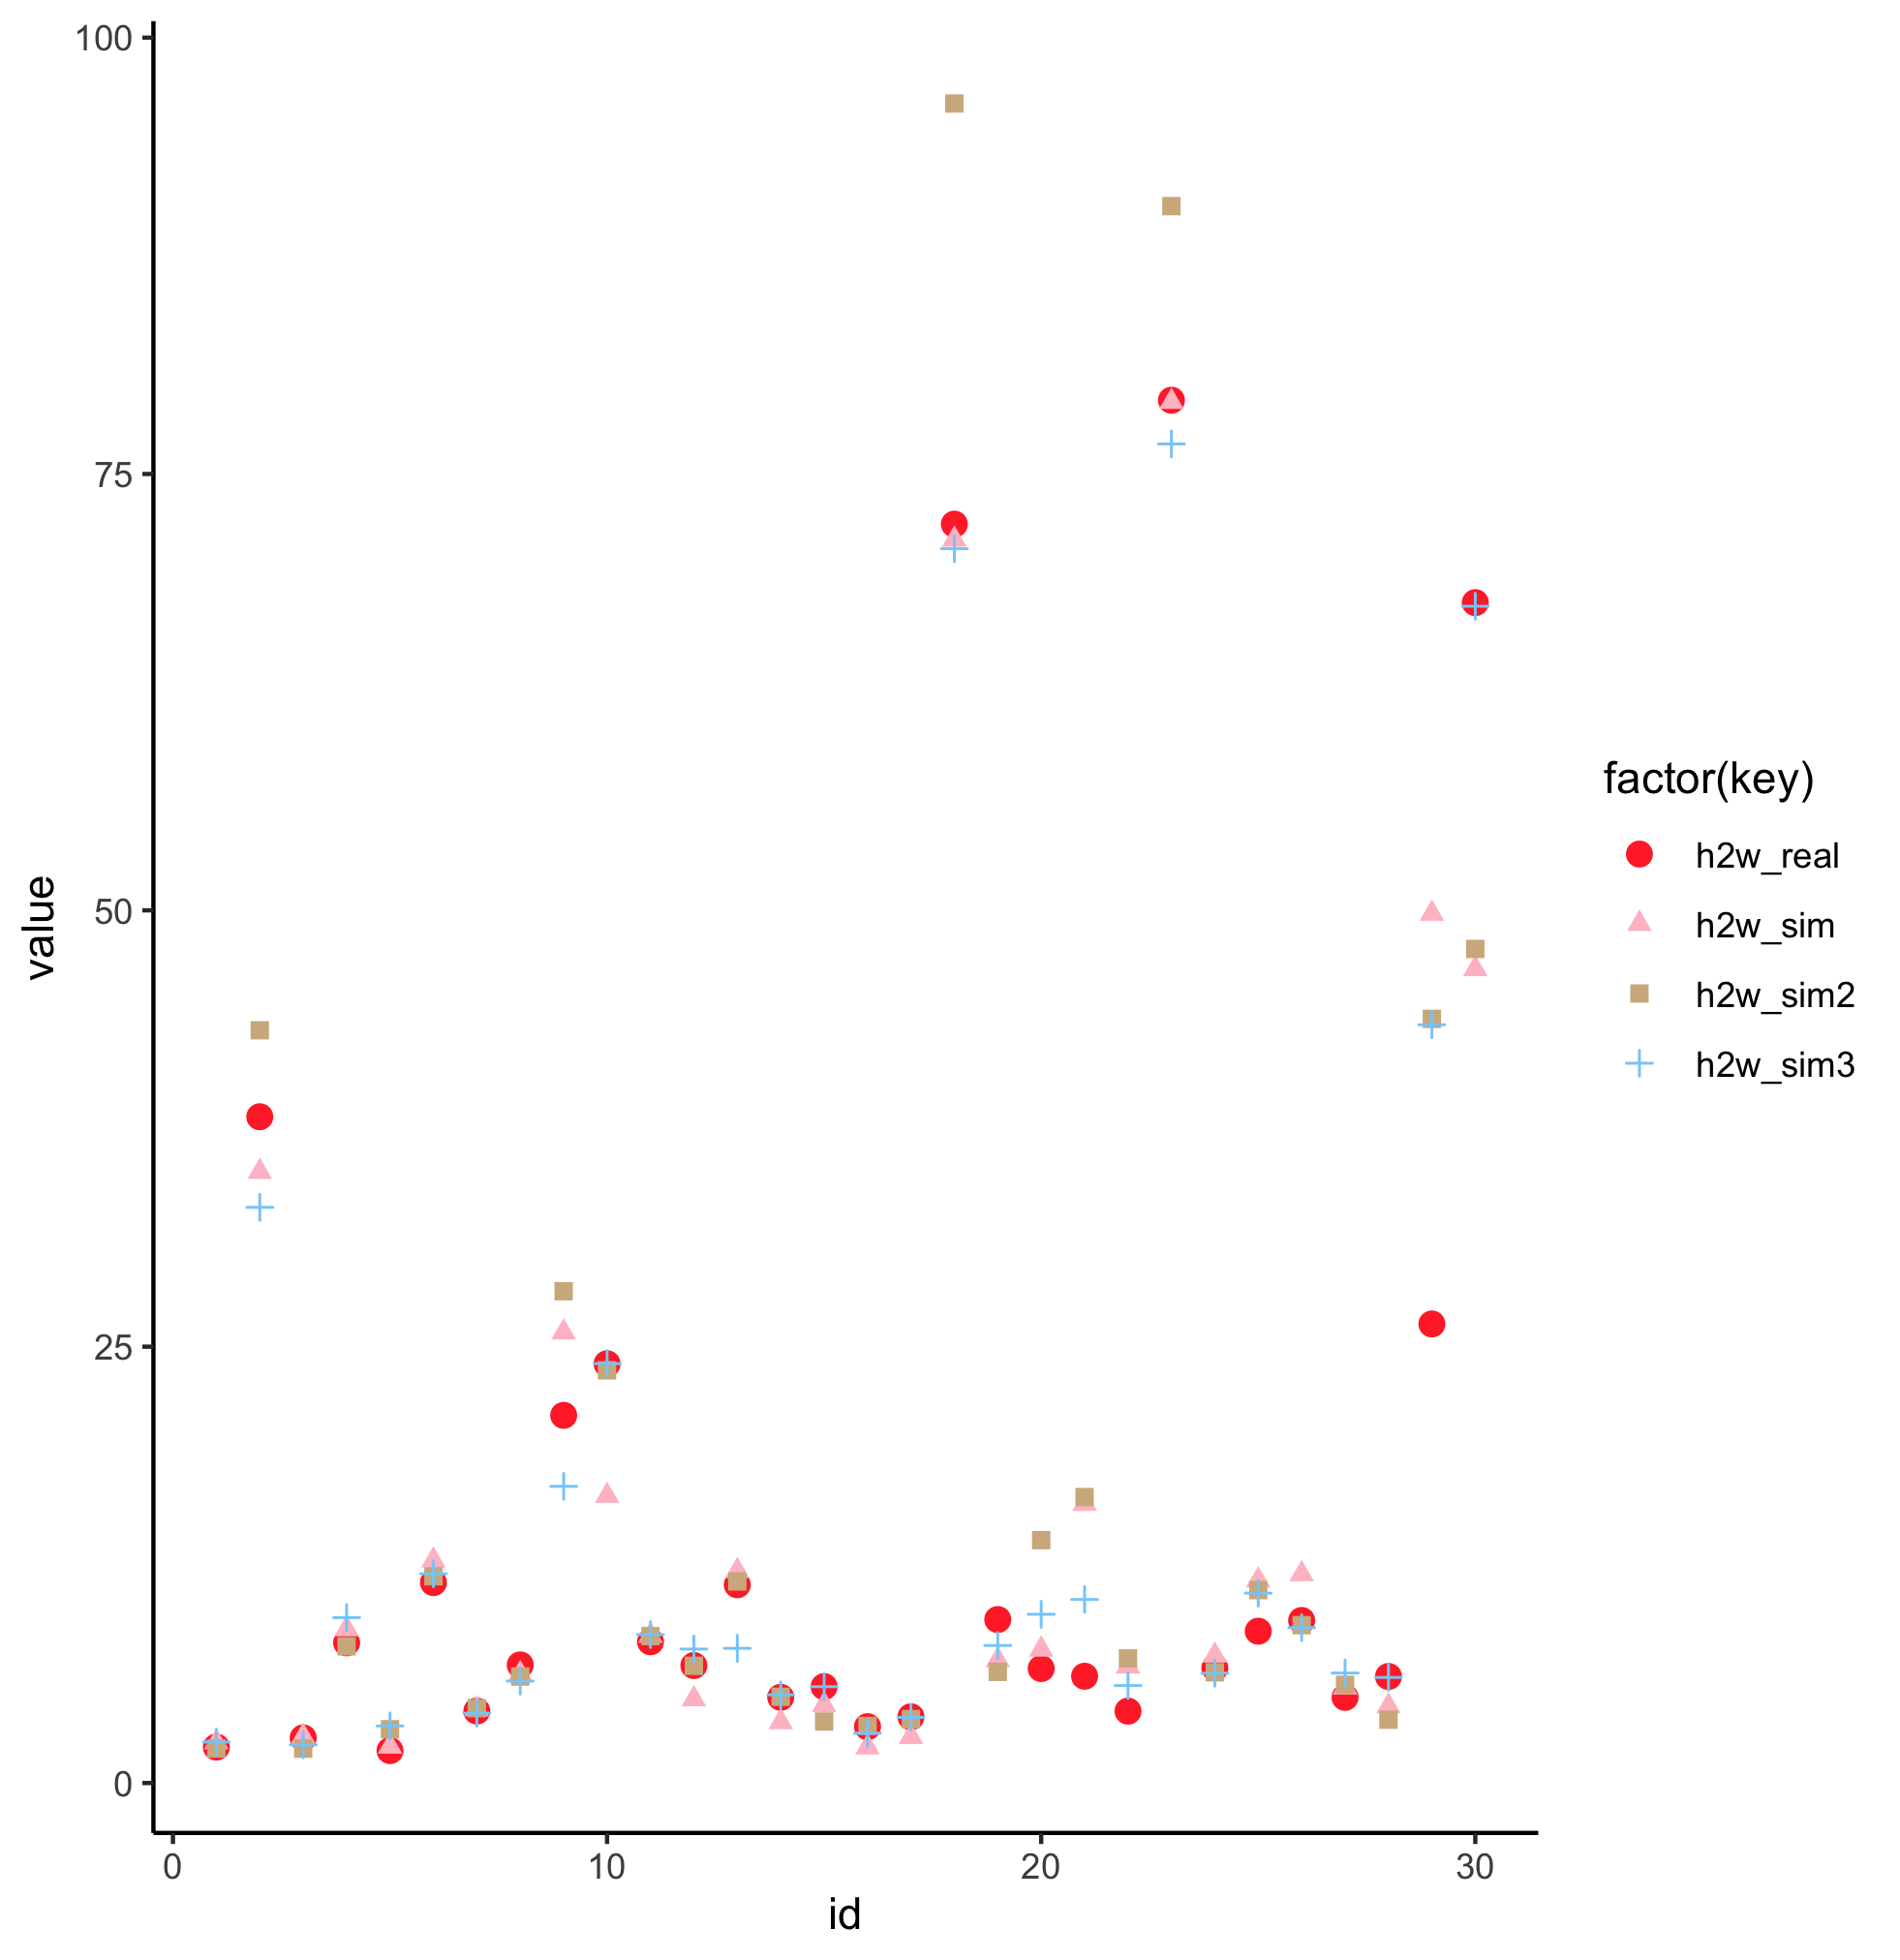
\includegraphics[width=8cm]{figure/sims.png}
    \caption{Exposure assessed for university, over the route home to university. The exposure is calculated as aggregating the NO$_2$ concentration along the route over the corresponding time span. The red dots indicate exposure assessed using real location, and others 3 times of simulated university locations and travel means.}
    \label{sims}
\end{figure}

\begin{figure}[h]
    \centering
    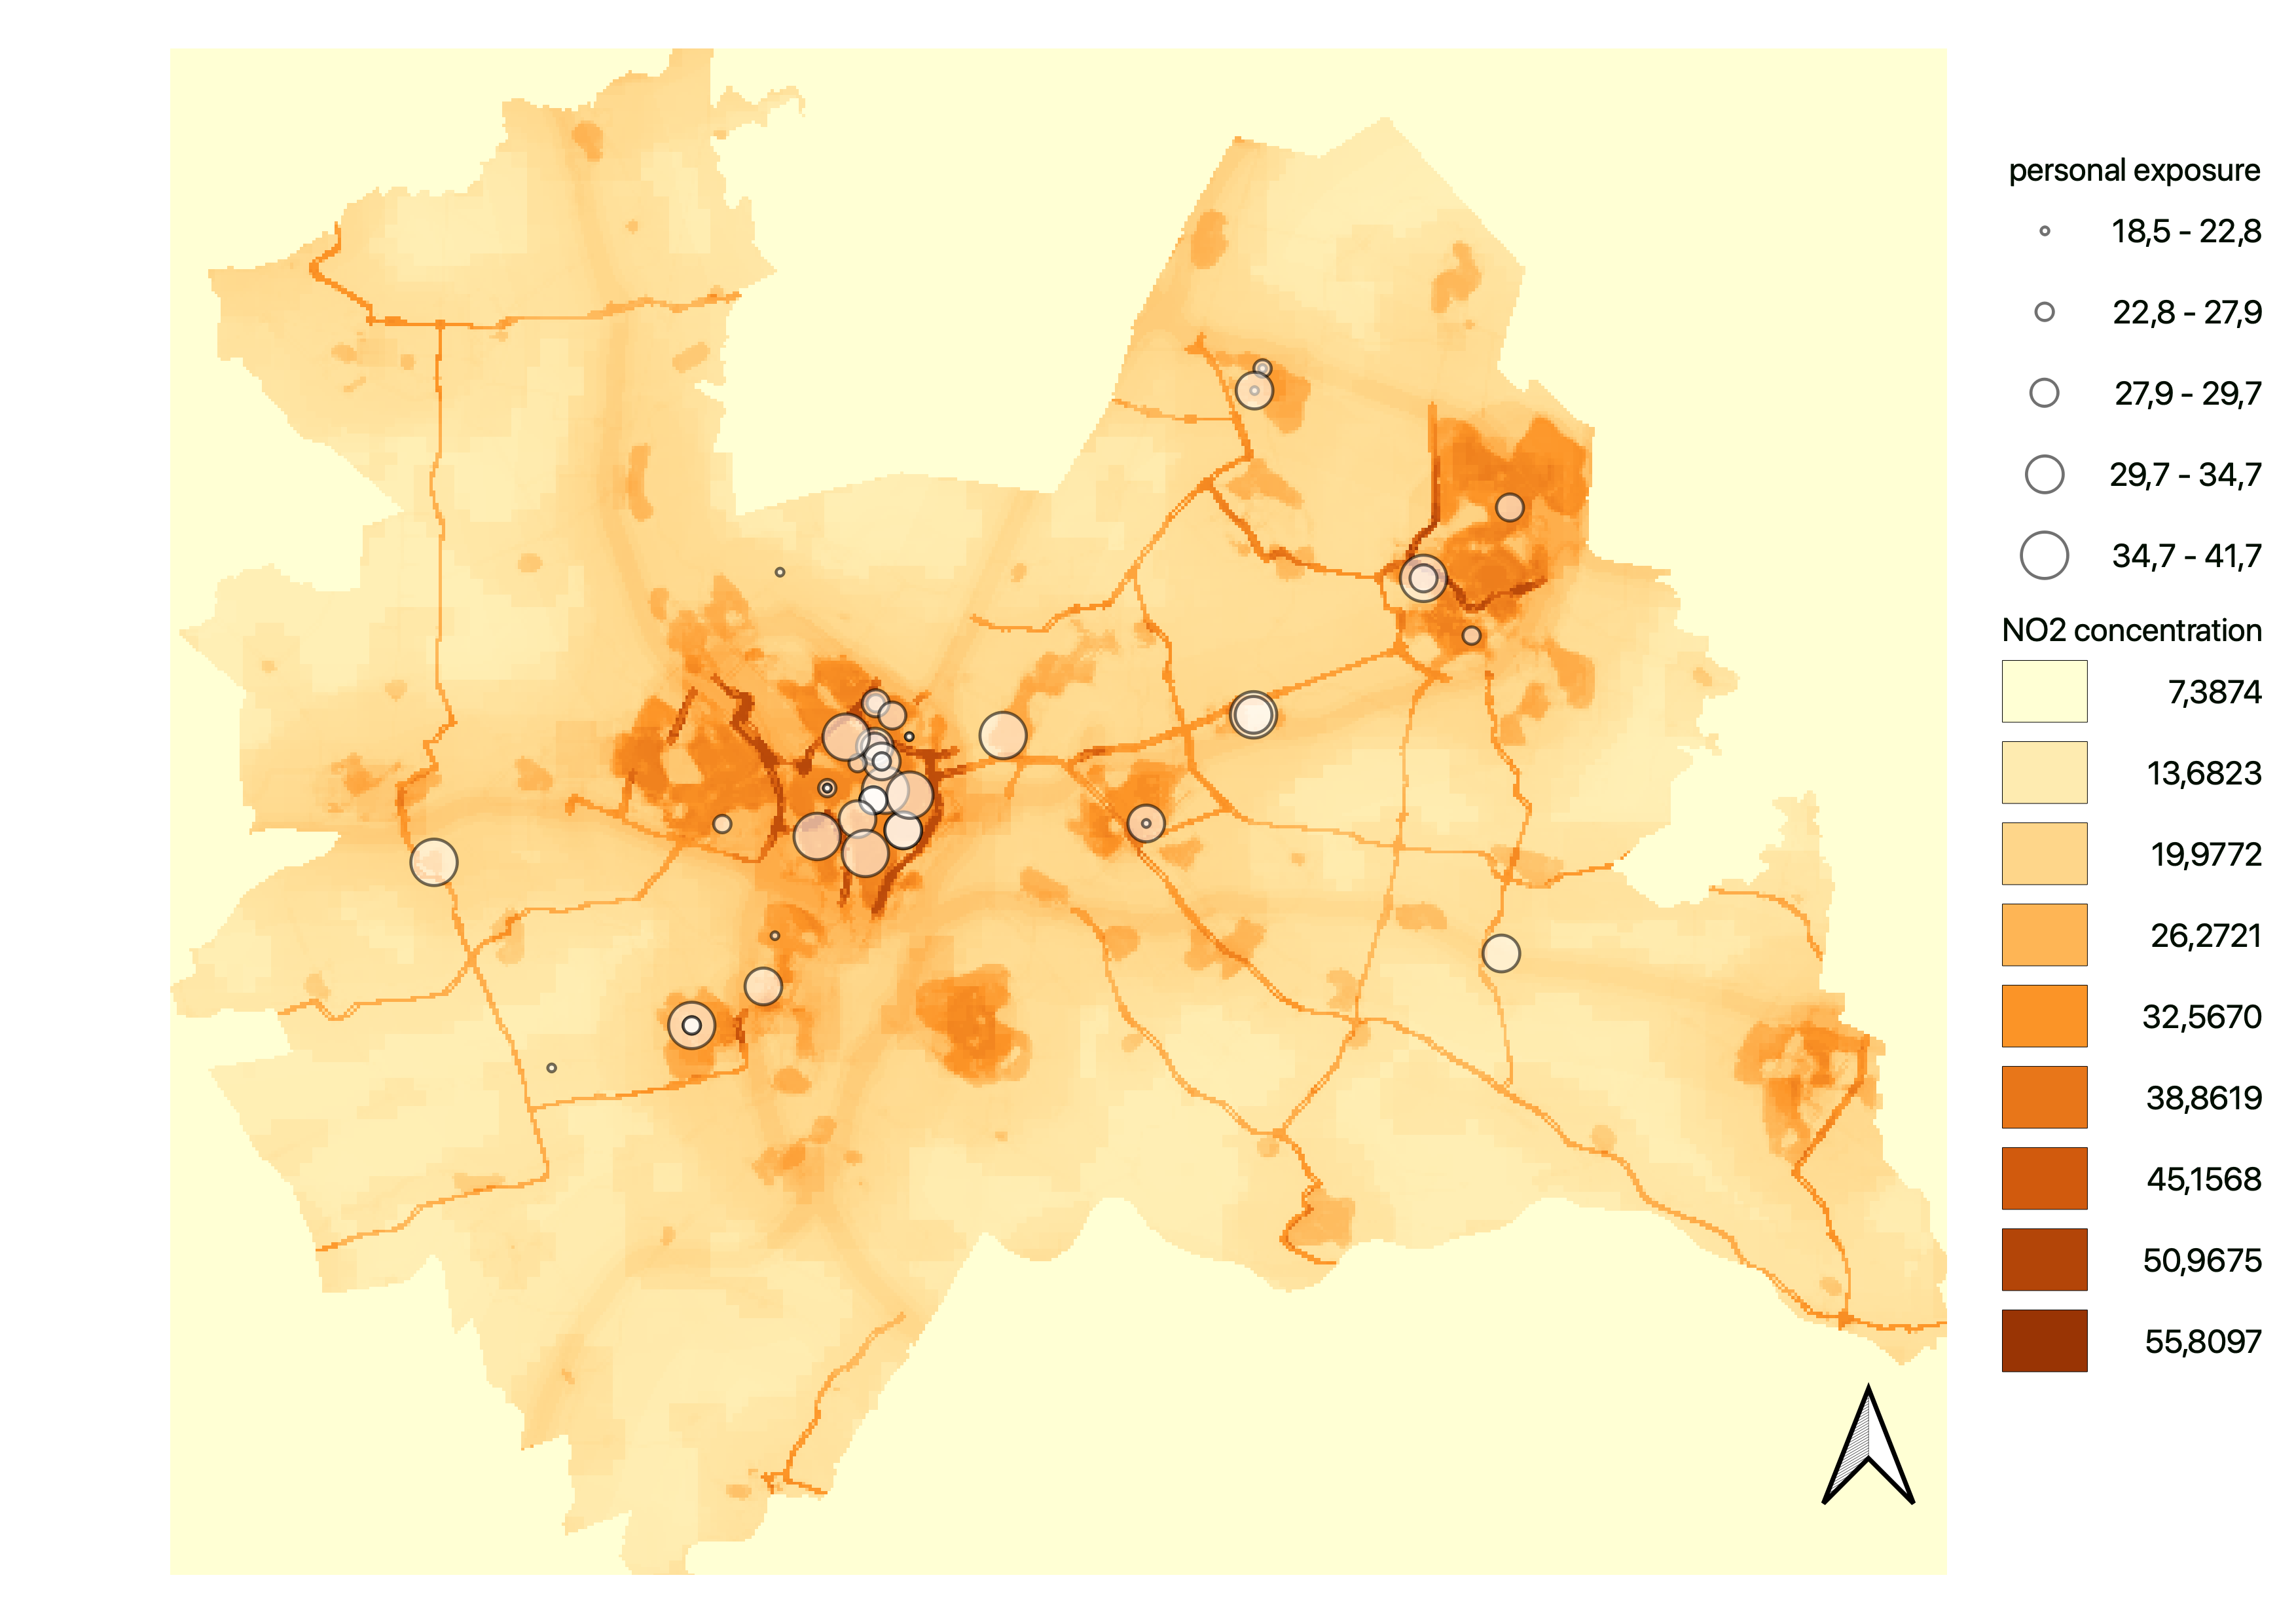
\includegraphics[width=8cm]{figure/exp49Utrecht.png}
    \caption{Exposure assessed for the population group "University students", it can be observed that high exposures do not necessarily occur for people with high concentrations on home locations. Background: annual mean NO$_2$ predictions.}
    \label{sims}
\end{figure}



\section{Discussion}
\label{sec:dis}
Trains are an important traveling tool for the population group full-time workers, half-time workers, and university students \cref{Uni_mode_dist}, which is the reason that we may implement the "travel by train" scenario. It is more complicated than other scenarios(as described in the section "Means of commuting" above). 
\begin{figure}[!h]
    \centering
    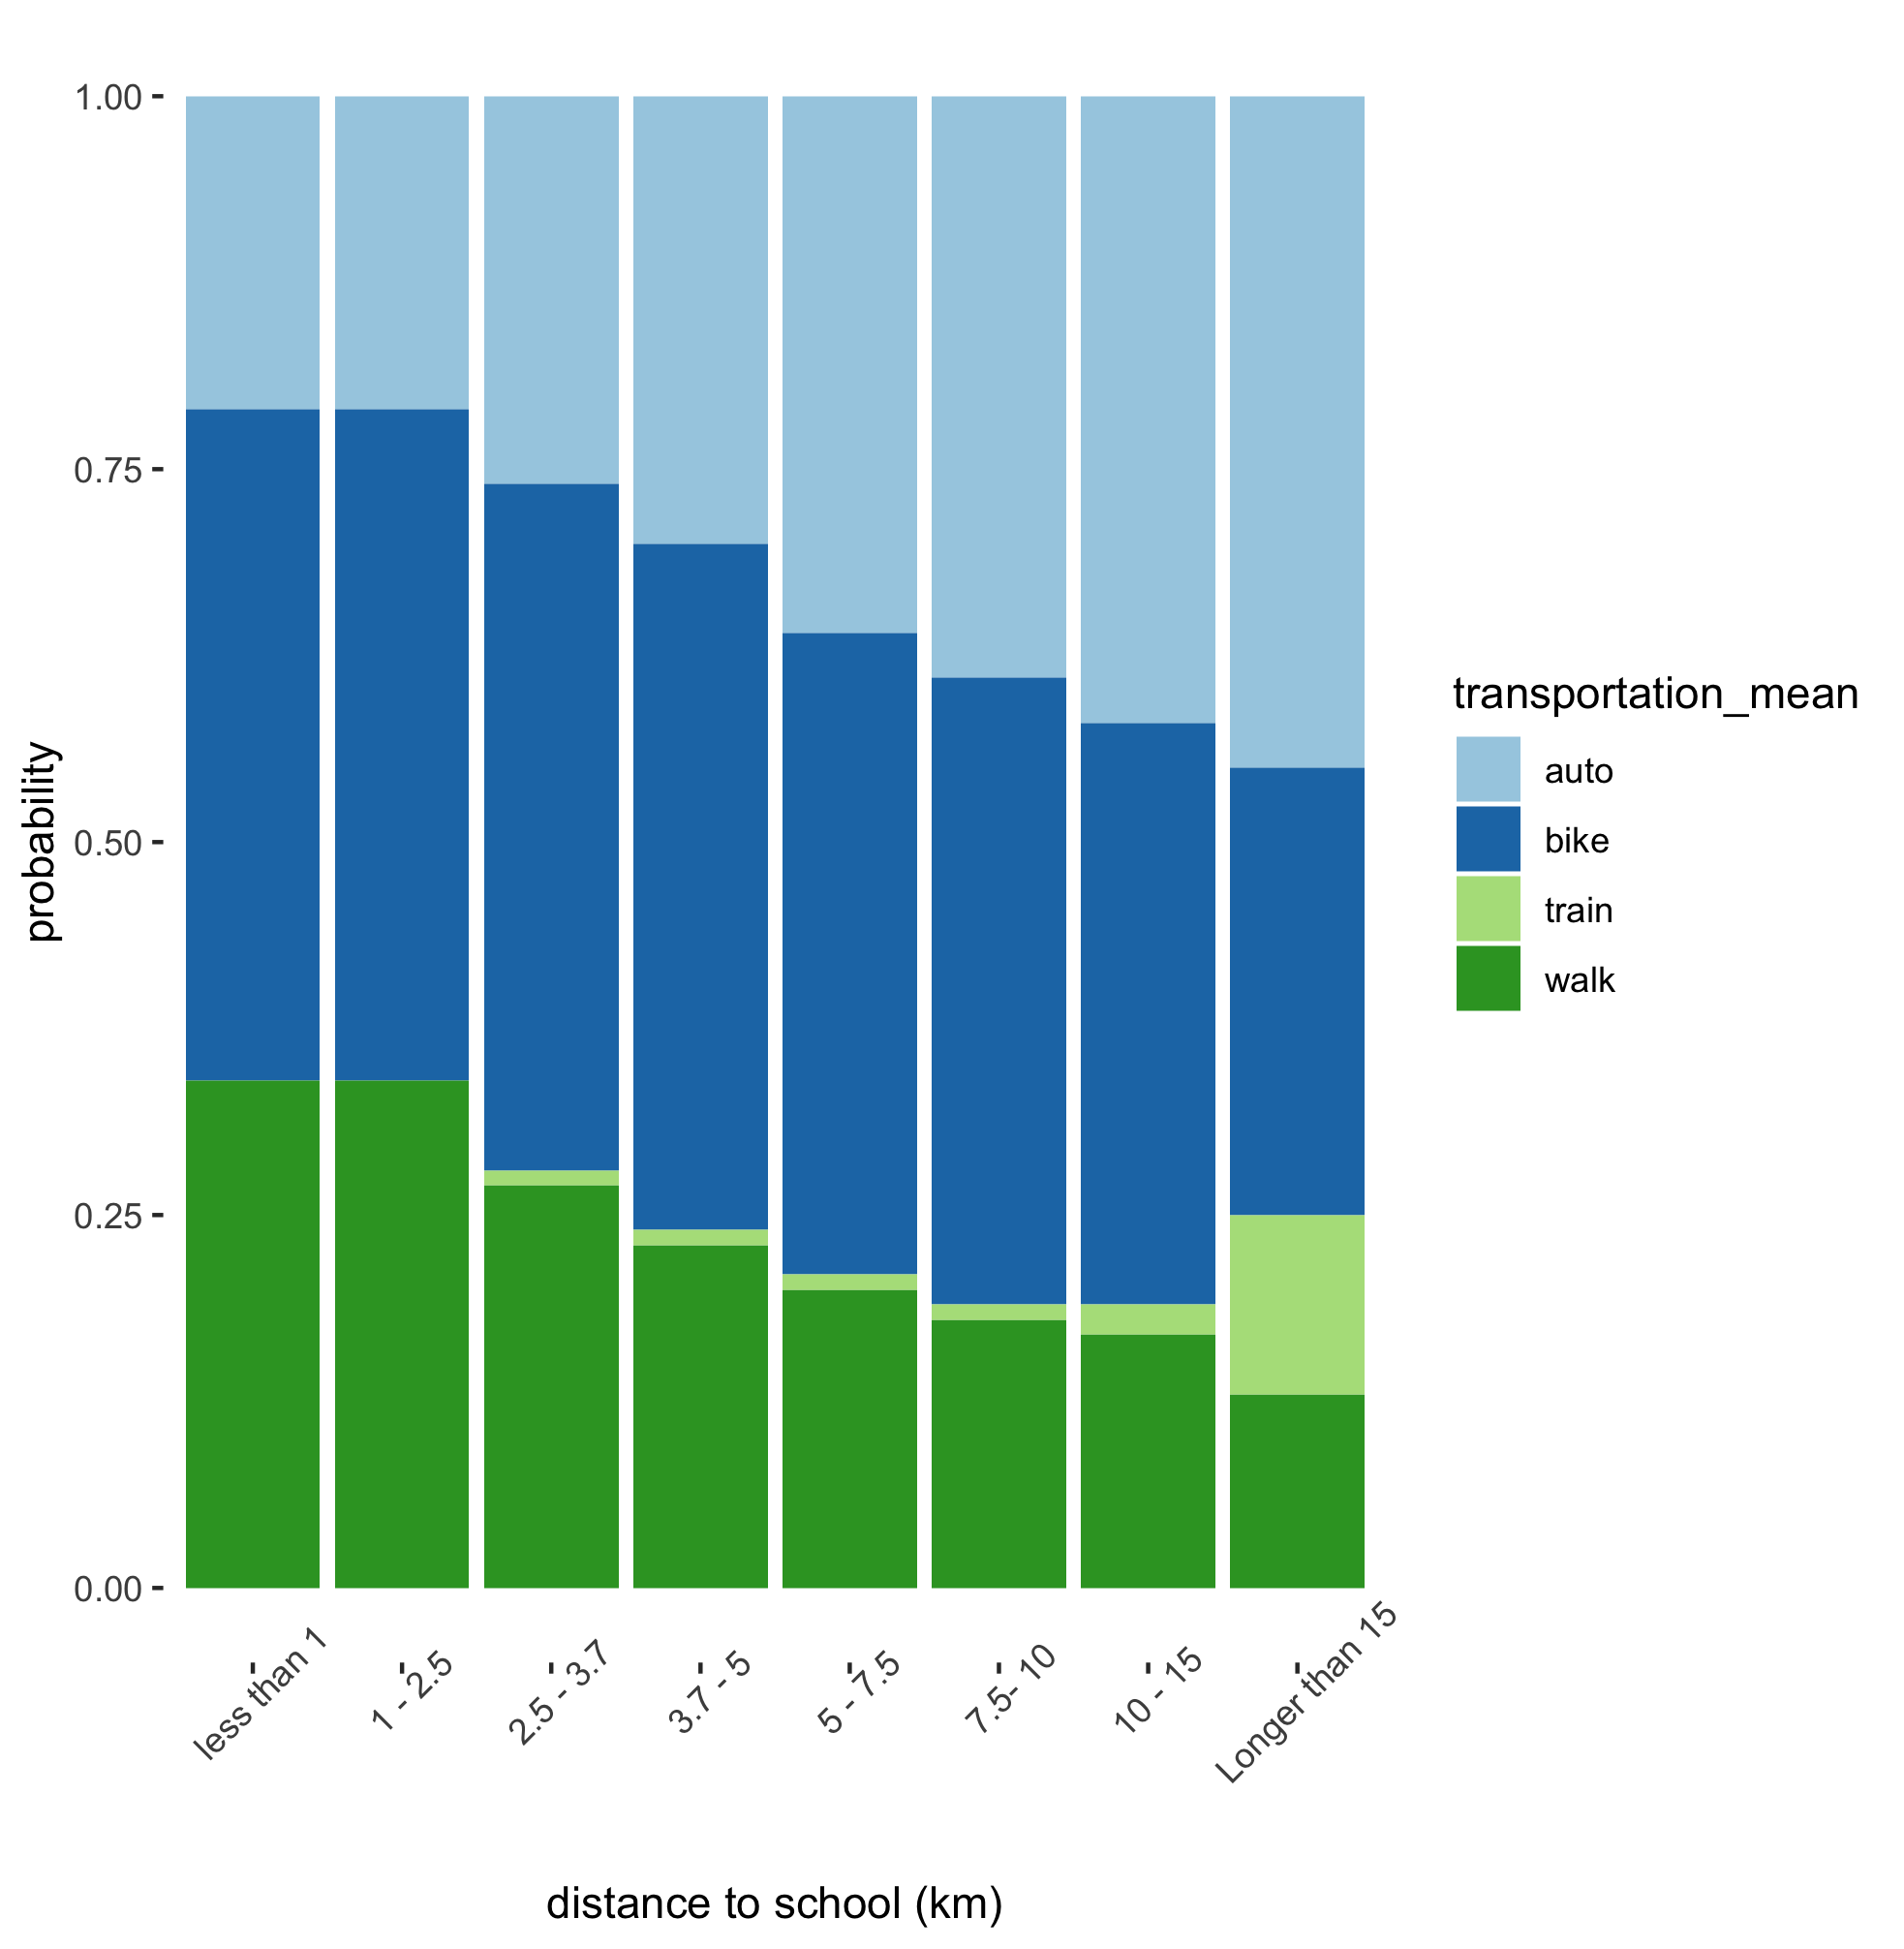
\includegraphics[width=8cm]{figure/ditance_vs_transmean_Uni.png}
    \caption{Probability of the transportation mean with regard to trip distance ranges for University students (older than 17). The trip distance ranges are re-scaled from the original travel distance. The transportation means are re-grouped from the transportation means in the Ovin survey.}
    \label{Uni_mode_dist}
\end{figure}

\section{Conclusion}
\label{sec:con}

The method can potentially be applied to long-term, large-scale air pollution exposure assessment and for many other exposure assessment tasks, for example Ozone and Particulate Matters. The flexible input makes it convenient to assimilate diverse data collections.


\newpage
\bibliographystyle{plainnat}
\bibliography{ref}


\end{document}

\begin{table}[!htbp] \centering 
  \caption{Example activity schedule 1, h2w means "home to work", and w2h means "work to home". The "bicycle" indicates the transportation mean, which is generated from the activity model. The integer part indicates hours, and the digits indicate minutes in percentage, e.g., 9.89 is at around 9:54 am. (54 = 89*0.6). } 
  \label{schedule} 
\begin{tabular}{@{\extracolsep{5pt}} cccc} 
\\[-1.8ex]\hline 
\hline \\[-1.8ex] 
 & start\_time & end\_time & activity \\ 
\hline \\[-1.8ex] 
1 & $0$ & $9.89$ & home \\ 
2 & $9.90$ & $10.19$ & h2w\_bicycle \\ 
3 & $10.20$ & $17.10$ & work \\ 
4 & $17.11$ & $17.39$ & w2h\_bicycle \\ 
5 & $17.40$ & $18.89$ & home \\ 
6 & $18.90$ & $19.89$ & sports \\ 
7 & $19.90$ & $23.90$ & home \\ 
\hline \\[-1.8ex] 
\end{tabular} 
\end{table}

\begin{table}[!htbp] \centering 
  \caption{Example activity schedule 2, for notations please refer to \cref{schedule}. "Auto" indicates all the other vehicles, of course, for U17, they are not driving themselves.} 
  \label{schedule2} 
\begin{tabular}{@{\extracolsep{5pt}} cccc} 
\\[-1.8ex]\hline 
\hline \\[-1.8ex] 
 & start\_time & end\_time & activity \\ 
\hline \\[-1.8ex] 
1 & $0$ & $9.33$ & home \\ 
2 & $9.34$ & $9.60$ & h2w\_auto \\ 
3 & $9.61$ & $16.43$ & work \\ 
4 & $16.44$ & $16.69$ & w2h\_auto \\ 
5 & $16.70$ & $18.19$ & home \\ 
6 & $18.20$ & $19.19$ & sports \\ 
7 & $19.20$ & $23.90$ & home \\ 
\hline \\[-1.8ex] 
\end{tabular} 
\end{table} 


\subsection{Implementation}
\begin{enumerate}
\def\labelenumi{\arabic{enumi}.}
\item
  Activities:
  \emph{Work-day activities:} 1) home, 2) home to work, 3) work, 4) work
  to home, 5) sports. The assumption for sports is that it occurs in the
  morning or evening, and it occurs either 1 hour before departure to
  work or 1 hour after come back home from work.

  \emph{Weekend activity}: 1) shopping, 2) random walk 
\item
  A \textbf{probailistic} model: the components below are probabilistic,
  and the distributions can come for activity surveys or literature.

  1) \underline{Time schedule:} please see section 2 for the activities.
  The departure times to work and back from home are probabilisitic. By
  default, a gaussian distribution is used (e..g with mean 8 and
  standard deviation 0.5 for going to work). In our implementation, the
  distributions of departure times are fitted (characterised) from human
  activity surveys (please see section 4 below). The distributions are
  fitted for each population group.

  2) \underline{Unknown destination locations:} For large-population
  activity modeling, it is commonly the case that the specific
  destination location (e.g. work location, sport centres) are unknown
  for each individual. However, the information for the entire locations
  (e.g. sport centres, work buildings, universities, schools) are
  becoming more comprehensive. In many countries, this part of
  information can be acquired from OpenStreetMaps. In this study, we
  select potential locations by proabilisticly sampling the maximum trip
  distance and only randomly select locations within the Euclidean
  distance of the maximum trip distance. If there is no destination
  points within the sampled maximum trip distance, the nearest
  destination point is used. The number of total selected destination
  points serve as an uncertainty indicator in the situation of unknown
  destination locations, in each simulation run.

  3) \emph{\underline{Means of commuting}} (currently: (train),
  autovehicles (car, bus, tram), bike, on foot): are deteremined based
  on travel distance. Based on the population group (e.g. school
  student) and the travel purpose (to school), the probability that a
  certain travel mean is taken is calculated (e.g. 0.3 for on foot and
  0.6 for biking, 0.1 for taking a bus or car and 0 for others),
  according to which a travel mode is sampled in each simulation. The
  commuting routes are queried from OpenStreetMaps.

  Note: {[}How is the train route calculated? If an agent (person) takes
  a train, it is assumed he/she will firstly walk or cycle to the
  nearest train station, and get off at the train station closest to the
  destination location. (\emph{to be considered}). I intend to firstly
  model within the Utrecht city, so all the destinations should be
  constrained to a certain distance, therefore the mode: train has a
  very small probability. This model may also be remove, then in
  implementation i can simply replace train with autovehicles{]} .
\item
  Implementation:

  Population group implemented are: school student (U17) , University
  student (students older than 18 years old, Uni), part-time worker
  (PW), full-time worker (FW).

  There is a conceptural default implemented in our model which is
  described in table 1. In our case-study (Utrecht) implementation, they
  are characterised from Dutch national activity surveys (OVin). The
  process is: 1) we select a profile (e.g. Univeristy student) and a
  purpose (e.g. go to work), 2) we fit the distribution of the selected
  data. 3) At each simulation, we sample one value from the
  distribution. Specifications are described below:

  \textbf{Destination location selection:}
\end{enumerate}
